\documentclass[11pt, a4paper, english]{book}
\usepackage{unir}
\usepackage[subpreambles=true]{standalone}

% Fore tables generated with www.tablegenerator.com
\usepackage[normalem]{ulem}
\useunder{\uline}{\ul}{}
\usepackage{tabularx}

\usepackage{float}
\usepackage{hyperref}

% To have sorted bibliography by last name
\usepackage[numbers]{natbib}

% Used to include code and config files
\usepackage{listings}
\usepackage{color}
\lstset{ 
  basicstyle=\footnotesize,
  breaklines=true,
  showspaces=false,                % show spaces everywhere adding particular underscores; it overrides 'showstringspaces'
  showstringspaces=false,          % underline spaces within strings only
  showtabs=false,
  tabsize=2
}

\graphicspath{ {images/} }

\title{Breakfastclub - Agent-based model simulation of a virtual classroom}
\author{Manuel Pasieka}
\date{\today}
\director{Michael Kickmeier-Rust, Elena Verdu Perez}
\nombreciudad{Valencia}

%---------------------------
%marges
%---------------------------
%\usepackage[margin=1.9cm]{geometry}
%---------------------------
%---------------------------
%---------------------------
%---------------------------
\begin{document}
\renewcommand{\listfigurename}{Figures}
\renewcommand{\listtablename}{Tables}
\renewcommand{\contentsname}{Table of Content}
\renewcommand{\figurename}{Figure}
\renewcommand{\tablename}{Table} 

\newcommand{\bb}[1][5mm]{\vspace{#1}}

\newcommand{\note}[1]{
  \fboxsep0pt
  \colorbox{green}{\begin{minipage}{\textwidth}
      NOTE: #1
  \end{minipage}}  
}

\maketitle

\frontmatter

\tableofcontents
\listoffigures
\listoftables

% Dissable paragrapth intention
\setlength{\parindent}{0pt}

\chapter{Abstract}

Agent-based models have proven to be a useful tool to study complex social phenomena.
In this work we have developed a simulation using an agent-based model of a virtual
classroom, simulating the behavior of students and adolescents in an autonomous
study group. The agent cognition is based on the widely used Big-Five personality
trait model, and agent behavior has been aligned with empirical studies showing
how specific personality traits correlate with academic success. The simulation
software was used to compare how different classroom compositions with an increasing
ratio of students with Attention-deficit hyperactivity disorder (ADHD) prototypical
personality traits affect the classroom dynamics. We found a very strong effect
of ADHD students on the mean classroom happiness and attention. Even a very small
number of ADHD students can cause a shift in the behavior of None-ADHD students,
decreasing their mean happiness and attention, in addition to more frequent classroom
wide quarrels.

\bb

The simulation software in addition with the data analysis pipeline is available
open source and under the MIT license. 

\bb

{\bf Keywords:} Agent-based model, Big Five, classroom, ADHD

\pagebreak


Model multi-agente son herramientas útiles para estudiar fenómenos sociales complejos.
Como parte de esta tesis hemos desarrollado una simulación multi-agente para
simular una clase virtual de un grupo de estudiantes autónomas. El modelo
cognitivo de los agentes se base en el modelo de personalidad de los cinco grandes
(BigFive), y genera un comportamiento que esta replicando resultados empíricos.
Para demonstrar las capacidades de la simulación hemos simulado como se cambia
la atención y felicidad media de una clase en función del número de estudiantes
con personalidades típicos de niños con trastorno por déficit de atención con
hiperactividad (TDAH). Hemos observado un efecto fuerte de los alumnos con TDAH
a la clase entera. Hasta un número muy bajo de estos alumnos produce una
reducción significante de atención y felicidad media, y además aumenta las
disputas en la clase.

\bb

La simulación y las herramientas de análisis de datos están disponible como open
source bajo de la licencia MIT.

\bb

{\bf Palabras Clave:} modelo multi-agente, Big Five, aula de clase, TDAH


\mainmatter

\chapter{Introduction}
This document is describing the Master Thesis developed by Manuel Pasieka as part
of the Master in Artificial Intelligence at UNIVERSIDAD INTERNACIONAL DE LA RIOJA, S.A.
2018-2019. \par

\bb

As part of the Thesis we developed an Agent-based simulation named
\textbf{Breakfastclub} (available at http://github.com/mapa17/breakfastclub) of
a virtual classroom in order to study the effect of different Personality Traits
on happiness and attention in a simulated class. This document is describing the
development of the project and the results achieved.

\bb

The document is split into the following chapters.
\begin{itemize}
\item This first chapter introduces the reader into the motivation behind this work and
its novelties.
\item The second chapter will discuss the state of the art of the methods and technologies
applied.
\item The third chapter lays out the initials objectives as well as their adaption
and final objectives of the Thesis.
\item The fourth chapter describes in detail the implementation and technical solution
to the proposed problem.
\item The fifth chapter is focused on the Data Analysis of the results generated.
\item The sixth chapter is providing a conclusion and summary of what has been
presented, as well as an outlook on possible future projects and extensions.
\end{itemize}

\section{Origin and Motivation}
The social climate of modern classrooms have been studied extensively in the past \cite{Anderson1982},
but common to many social studies, only the results of few empirical studies have been modeled
successfully. This is changing, and in part because of the availability of
computational methods and the availability of public data. Methods from statistical
physics are applied more and more successfully in studying complex social systems
(an extensive review on the topic can be found in \cite{Castellano2007}).

\bb

One method that has proven especially useful in studying social systems are
\textbf{agent-based models}\cite{Jackson2017} that are a special type of multi-agent systems
which models the behavior of individuals and can be used to study their interactions
and emerging social behavior.

\subsection{Simulations in the Social Sciences}
In their work \cite{gilbert2005simulation} the authors give a short history of
simulations in the social sciences. They explain different reasons why simulations
can be applied with different objectives,ranging from better understanding a social
system, to prediction, to substitute human experts, as training tools, entertainment
or as tools to for discovery and formalization of models.

\bb

Specially the later applications of simulations in the social sciences are interesting
to us, as traditional approaches to understand complex phenomena in the social sciences
have been focused on comparing the results of empirical studies to hypothesis
generated with theoretical models.

One of the difficulty with this approach are the increasing costs of such studies
in face of more and more complex models. The growing complexity and the degree of
freedom of these models, demand a equally growing sample size increasing costs and the
resources needed to generate results that can be used to verify and reject hypothesis
in order to improve the models.

\bb

Figure \ref{Cycle-TSE} demonstrates how simulations can be used to support
the discovery and improvements of new models and theories. Given a theoretical model
one can produce hypothesis that are used to situate a simulation, providing the initial
conditions and input parameters for the simulation. The simulation models is than
run to produce concrete predictions, that can be compared to experimental studies.
The overlap between the prediction and measured results is than used to form new
hypothesis that can be used to improve theory and future models.


\begin{figure}[H]
    \makebox[\textwidth][c]{%
    \begin{minipage}[t]{10cm}
        \centering
        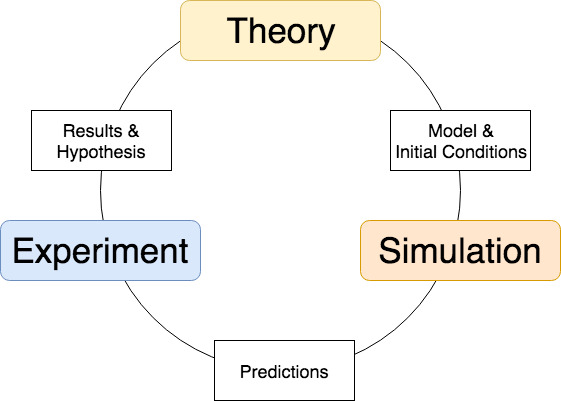
\includegraphics[width=300pt]{Theory-Simulation-Experiment}
        \caption{Cycle of Theory, Simulation and Experiment }
        \label{Cycle-TSE}
    \end{minipage}    
    }%
\end{figure}

\bb

As will be described in more detail later, our work is focused on studying the group
dynamics of children in a classroom, in particular that of a autonomous study group.

In order to achieve this, we split the task in two goals
\begin{enumerate}
    \item Develop a flexible and extendable agent-based model of a virtual classroom
    \item Study how different personality traits effect attention and happiness of individuals and the group as a whole
\end{enumerate}


\chapter{State of the art}

\section{Agent based models}
What are Agent based models and why they are interesting for studying social interactions in groups

\section{Big Five Personality Trait model}

\section{Agent Logic???}
Where to talk about agent logic and possible ways to define an agent in a multi-agent system?

\section{Simulation Environments}
Mention Unity3d, but as well NetLogo and other environments.


\chapter{Objectives and Methodology}
The main objective of this Thesis is the development of a simulation using an
agent-based model that is capable of simulating students in a virtual classroom.

\bb

As it is typical for projects beyond certain size, the objectives and scope had to
be adapted according to the progression of the project after the initial planning phase.
This chapter describes the initial envisioned objectives as well as the objectives
reached with the final version of the thesis.

One of the initial objectives of the thesis was to develop a simulation environment that
could be used interactively as well as a closed loop simulation (i.e. once defined
and setup would run without any user interaction until a defined state is reached).

In addition as the simulation is based on Unity3d, the Machine Learning Package
was intended to be used to implement agents trained using a Reinforcement Learning approach.

Because of time constrains the interaction and ML-Agent features have not been included
in the final version developed during the Thesis, but are included in the last chapter
on the outlook of the project.

\section{Particular Objectives}

The objectives for the final version based on the resources and time available
have been the following:

\begin{itemize}
    \item \textbf{Closed Loop Simulation:} Implementation of Unity3d based virtual
    classroom simulation, including a 2D top down visualization.
    \item \textbf{Psychological agent model:} Development of a psychological model
    governing the behavior of agents that is based on empirical and theoretical grounds.
    \item \textbf{Deterministic Simulation:} The closed loop simulation should be
    deterministic and the random components should be seedable, making it possible
    to reproduce results of previous simulations if the same seed is provided.
    \item \textbf{Simulation and Classroom configuration:} The simulation as well
    as well as the psychological profile of the classroom should be easily configurable
    and alterable without the need to modify the simulation software.
    \item \textbf{Agent and Classroom based analysis:} As part of the data analysis
    it should be possible to analyze the behavior of individual agents (i.e students)
    as well as the average of the complete classroom (i.e. group).
    \item \textbf{Comparison of pre-defined psychological classroom profiles:} Based
    on empirical pedagogical studies a defined set of psychological interesting classroom
    profiles are compared to each other.
\end{itemize}

\section{Methodology}
The development of the simulation was following an \textit{agile software development}
principle in which based on two prototypes, and many small iterations the final
software was developed.

\bb

In order to keep track of the project progress and open tasks, the issue and project
management system that is part of Github was used. There we defined two main milestones
for the final simulation, describing goals and associated tasks.
During the development progress, any arising change was documented and the associated
code changes have been managed as Github issues.

\bb

Concerning the agent mechanics and simulation parameters, an iterative process was
pursued. The behavior of agents was observed manually using the interactive simulation
for any abnormal or undesired behavior. Once an issue was identified, the agent logic
was adapted to resolve the issue, and its correctness verified observing the
simulation process.

\bb

Simulation Parameters have been chosen using the data analysis scripts developed
as part of the thesis (see chapter \ref{Chapter:DataAnalysis}). The behavior
of individual agents, as well as classroom aggregates have been used to find
the simulation parameters used to perform the study (Simulation parameters are included
in the Appendix). The parameters have been tuned using three classroom profiles,
following different objectives.

\begin{itemize}
    \item \textbf{Normal classroom:} A classroom with 30 students having a 'normal'
    personality profile, has been used to define thresholds like noise, happiness
    and motivation increases.
    \item \textbf{Test classroom:} A special test class containing different types of
    personality profiles has been used to verify that simulated agent behavior is
    corresponding to results gathered in empirical studies.
    \item \textbf{Random classroom:} A special classroom with students having random
    personality profiles was used to maximize the difference in happiness and attention
    between different agents.
\end{itemize}


\chapter{Development}
This chapter describes in detail the main components of the simulation and how
they where implemented. How and why certain decision have been taken and alternative
solutions.

The project was developed in an iterative fashion, following with a first Prototype
after the initial literature research and evaluation of alternative simulation frameworks
(see \ref{StateOfTheArt}).

\section{Agent-based model}
As described briefly in the chapter on the State of the Art (\ref{StateOfTheArt})
a agent-based model is a multi agent simulation with a special focus on the interaction
and resulting group dynamics of its agents. The main components of a Agent-based
model are the following:

\begin{itemize}
    \item \textbf{the environment:} The environment is a strictly
    defined space in which the agents can move and interact with each other as 
    well as with other objects that are part of the environment. 
    \item \textbf{the agents:} The agents are autonomous dynamic systems with a
    set of sensors and actors that interact with each other and with the environment.
    \item \textbf{the simulation mechanics and agent logic:}  The simulation mechanics
    controls how agents interact with each other, how the environment changes
    as of actions of the agent or external factors (e.g. a simulation protocol defining
    a change in the environment). The agent logic governs the dynamic cycle between
    the agent, other agents and the environment. It defines how internal states change,
    and which behavior the agent should perform.
\end{itemize}

\subsection{Unity3d}
Unity3d[NOTE: REF] is a Computer Game Engine that has been used to develop not only
AAA (i.e. high quality [NOTE: definition]) computer games but as well is continuously
applied more and more to build simulations for commercial and academic purposes.
Unity3d is distributed under various licencees, including a Free use license, which
enables its use for Indie Game Developers as well to be applied in Academia without costs.
For our purposes Unity3d is a generic Simulation Framework that provides the tools
to create virtual 3d environments, a physics engine, a User Interface and autonomous
agents.

The simulation is implemented as a Unity3 application with a single scene that is
dynamically generated based on the simulation and classroom configuration.

All objects (Agents and Tables) in the classroom are Unity GameObjects that are
updated in defined sequence with a constant rate of 1 Hz. The agent logic is therefor
running in discrete steps, although the underlying Unity3d engine is executed
continuously (as much as this is possible on a discrete computer system).

Although not completely separated, Simulation Logic is split from game content
like Sprites (i.e. Images), Animations and other visual elements. The Simulation
Logic is implemented as C\# scripts that interface the Unity3d Framework.
During the development it was taken care to separate the Unity3d specific elements
from the rest of the simulation logic, in order to reduce dependence and make it
possible to port the Simulation Logic to other platforms.

\subsection{The environment: a classroom}
In our case the environment is classroom that contains multiple tables for
students to study individually and in small groups. In addition the environment
is modeling the noise that is accumulating in the classroom resulting from the
different actions performed by the agents.

Agents are moving about in the classroom as part of the various actions they perform.
The Unity3d Navigation Agent Infrastructure is used to control the movement of agents,
including path finding and collision control.

The noise model implemented, is accumulating the noise produced by the different actions
performed by all agents in the classroom. Different Actions produce different amount
of noise depending on the simulation configuration.

\label{agent}
\subsection{The agents: school children}

\begin{figure}[]
    \centering
    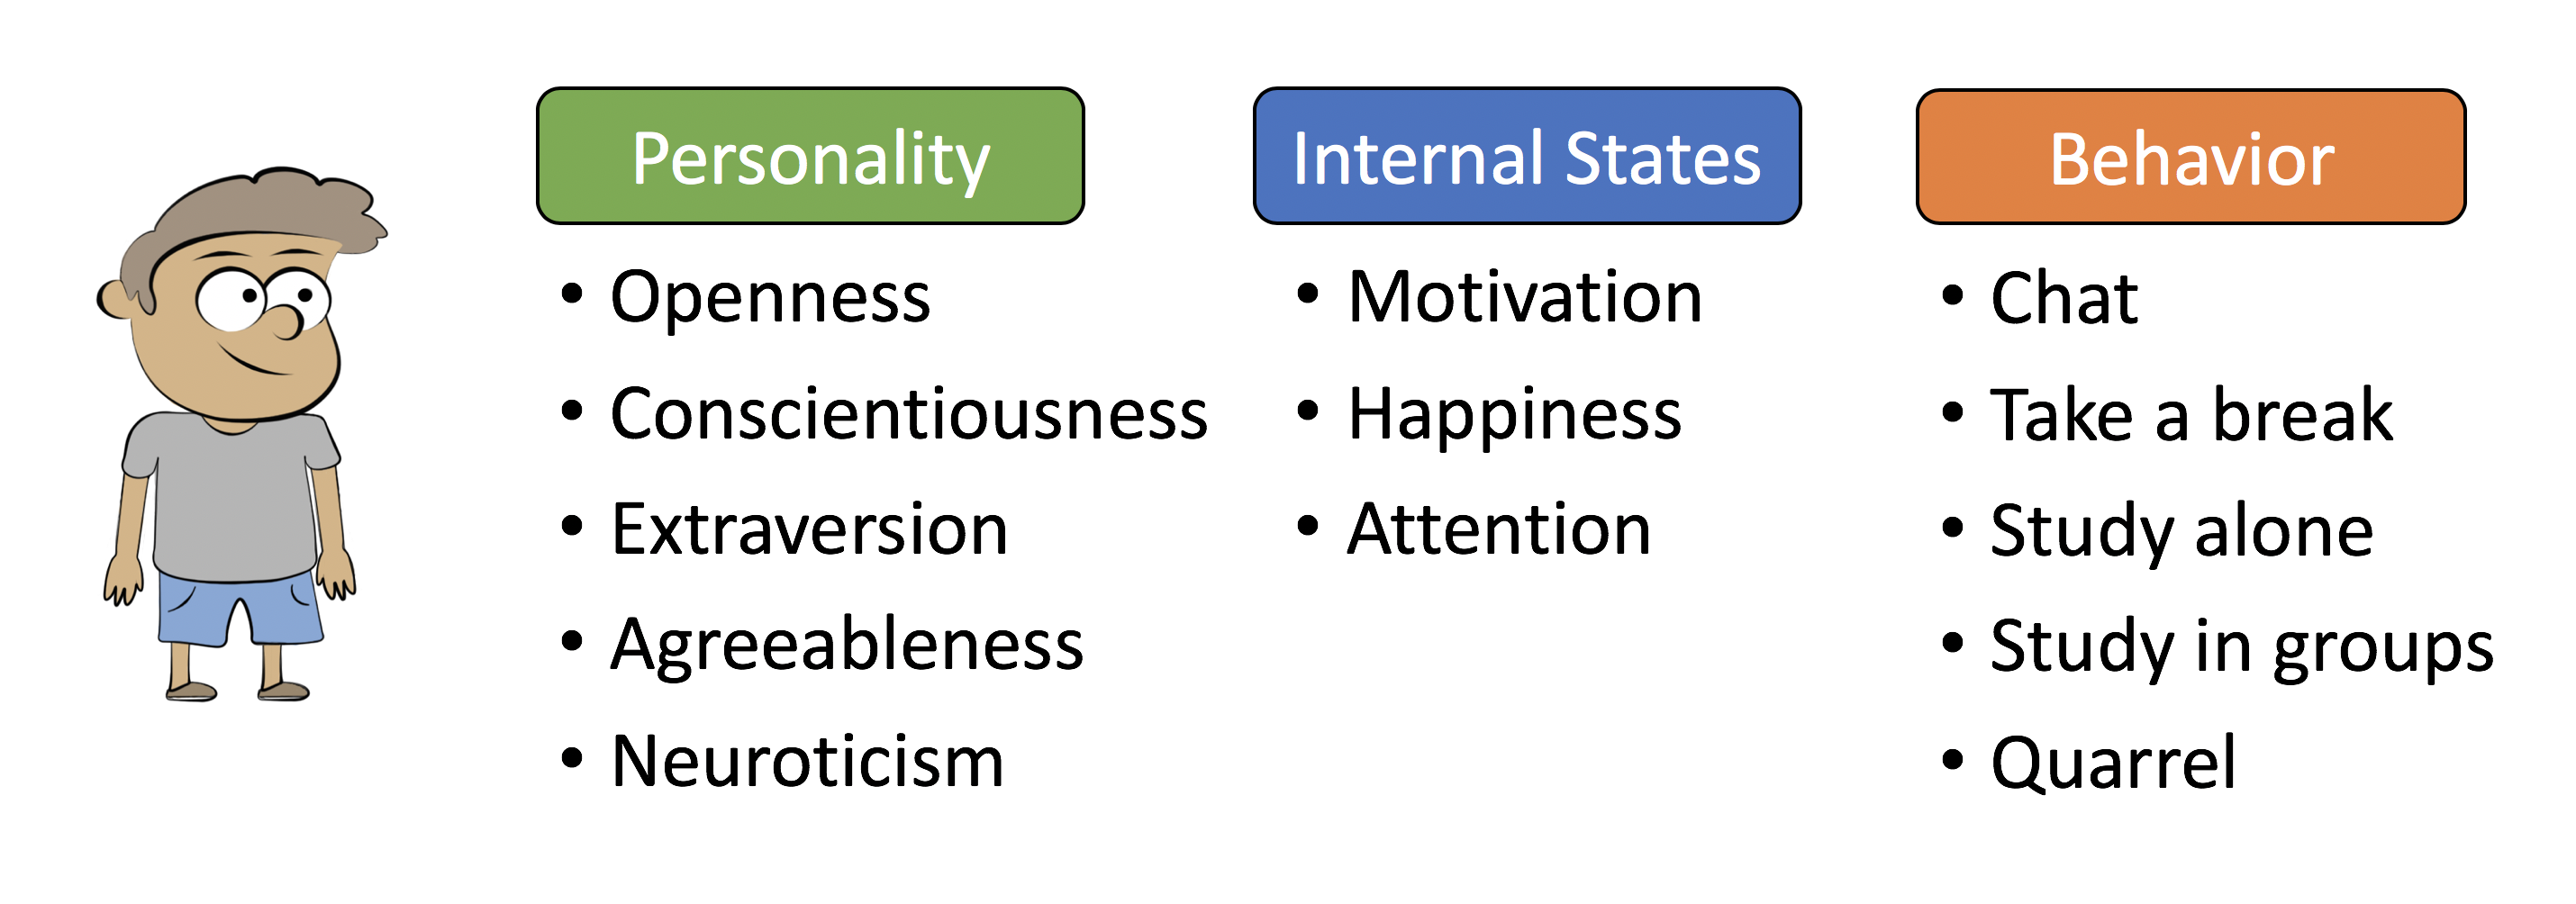
\includegraphics[width=400pt]{AgentOverview}
    \caption{Agent Overview}
    \label{AgentOverview}
\end{figure}

The agents are modeled to simulate school children of no specific age or physical
property. Instead agents are characterized by their personality traits based on 
the Big Five Personality Traits model (see \ref{BigFive}). In addition agents have
several internal states and a set of possible behaviors they can perform (see \ref{AgentOverview}).

The internal states modeled by the agent are \textbf{motivation} to study, \textbf{happiness}
and \textbf{attention} during studies.

The behaviors available to the agents fall into one of three different types, being
either educational, recreational or the conflict.

\begin{itemize}
    \item \textbf{Chat:} Agents chat with another random selected agent in the classroom.
    \item \textbf{Take a break:} Agents take a break and start a random walk through the classroom.
    \item \textbf{Quarrel:} Agents start to quarrel with another random selected agent in the classroom.
    \item \textbf{Study alone:} Agents sit down on one of the individual tables and learn by themselves.
    \item \textbf{Study in groups:} Agents take a spot on a group table and study with the other agents on the table.
\end{itemize}

All possible actions, are in one of the following states at each moment in time

\begin{itemize}
    \item \textbf{Inactive:} The action is not active at all (This is needed because of implementation details). 
    \item \textbf{Transition:} The agent is walking towards it needs to in order to perform the action.
    \item \textbf{Waiting:} The agents is waiting for either some response of another agent in order to perform the action.
    \item \textbf{Executing:} The agent is actively performing the action.
\end{itemize}

As the agents behavior depends on the internal states but as well is effecting them,
each agent itself is a \textbf{dynamics systems} that is governed by the agent logic, based
on the personality profile of the agent (see a visualization of this cycle in figure \ref{AgentDynamics}).

\begin{figure}[]
    \centering
    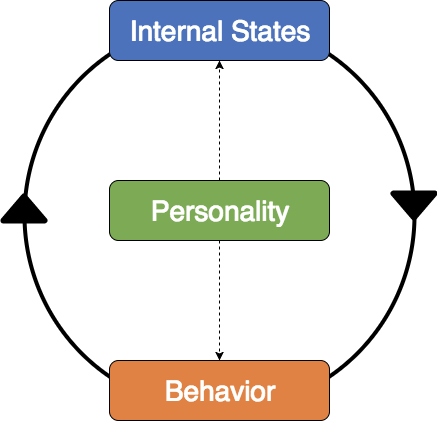
\includegraphics[width=200pt]{AgentDynamics} 
    \caption{Agent Dynamics}
    \label{AgentDynamics}
\end{figure}

\subsubsection{Dynamic Systems}
As mentioned in the introduction, agent-based models are focus on the interaction
\textit{between} components of the simulation. The complete system is therefore
the result of the interaction of multiple dynamic systems (i.e. agents and environment)
(see figure \ref{GroupDynamics}). 

\bb

This \textbf{multi level dynamic system} can express very sophisticated behavior and dynamics,\
making it one of the main reasons agent-based models are such a powerfully tool to study
real world phenomena. One of the most curious aspects of complex dynamic systems
are \textbf{emergent phenomena}\cite{Corning2002} which describes aspects of the
complete system (i.e. classroom), absent in the individual (i.e. children) components.

\bb

One examples of emerging properties is the \textit{wetness} of Water that only appears in a
ensemble of many water molecules, not present in a single individual molecule. 
Another famous example is \textbf{Cowans Game of Life}\cite{Adamatzky2010}
that shows the almost infinite complexity generated by a cellular automata simulating
black or white cells on a infinite grid. Constructs generated by the simulation
have emerging properties like \textit{self replication}, \textit{finite} and
\textit{infinite cycles} and many more. None of those behaviors are obviously deducible
from the initial basic interaction rules. Instead those properties emerge in the
interaction between the rules 'agents' (using agent in an amplified sense here)
following basic rules.

\begin{figure}[]
    \centering
    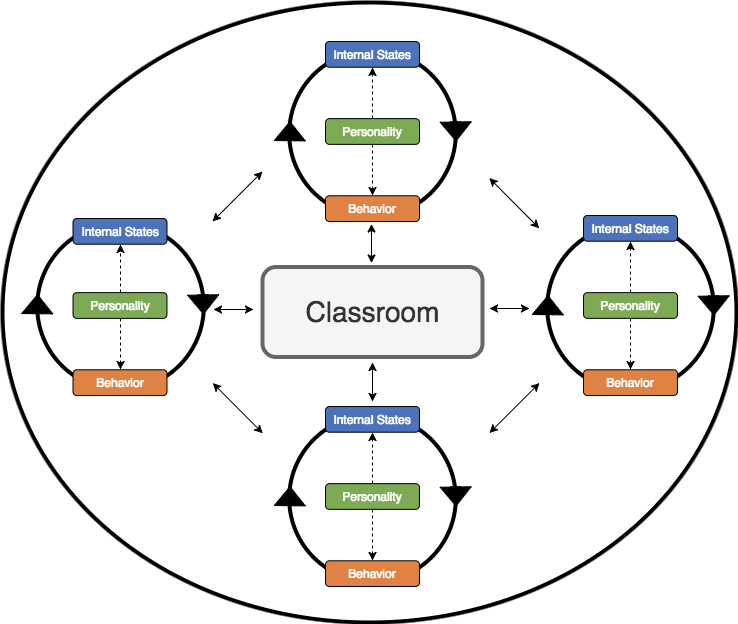
\includegraphics[width=200pt]{GroupDynamics} 
    \caption{Group Dynamics}
    \label{GroupDynamics}
\end{figure}

\subsubsection{Agent homogeneity}
One axis along which to classify agent-based models is agent homogeneity\cite{Pudane2017}.
In homogeneous agent models all agents share the same characteristic's and agent logic.
Heterogeneous agent models on the other side can differ in the agents logic, its behavior
or based on some parameters in its configuration.

In our case the simulation contains heterogeneous agents that differ, based on parameters
in their Personality Traits. 

\label{BigFive}
\section{Agent Personality Traits}
As described earlier each agent is a dynamic system that in which the internal states
interact with the agents behavior. Those interactions are governed by the agent logic
witch is based on the \textbf{Personality Traits} of the agent.

It is not novel to use personality traits in ABM, but previous works\cite{Gautam2009}
modeled very abstract personality traits that have no relation to the real world.

We therefore where careful, to chose an established and widely used personality traits model.
The \textbf{OCEAN} personality trait model\cite{Tupes1961}, common known as the \textbf{Big-Five}, has been developed
in the 1960s and has since been used in applied and theoretical psychology.
It is based on factor analysis of empirical studies (mostly self description of patients about their
behavior and self image).

Its name is derived from the five orthogonal dimensions which are used to describe
the personality of an individual, where the extremes of each dimension are associated
with typical behaviors or thought patterns (see figure \ref{OCEAN-Model} for a graphical
representation).

A short description of the different dimension has been taken from\cite{Ehrler1999}
(see table \ref{OCEAN-Model-table} ).

Although the personality traits of a person could change over time, there is strong
evidence (\cite{Soldz1999}, \cite{Cobb-Clark2012}) that the personality traits of
the big five model stay more or less constant over a long period of time or even
the complete life of an individual.

\begin{figure}[h]
    \centering
    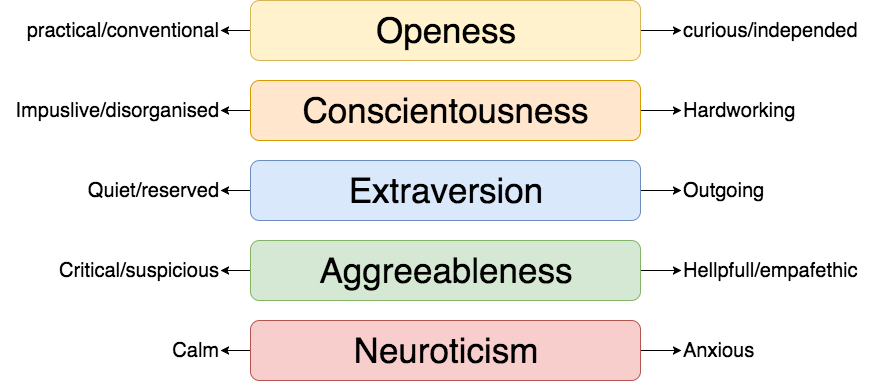
\includegraphics[width=400pt]{OCEAN-model} 
    \caption{OCEAN Model}
    \label{OCEAN-Model}
\end{figure}

\begin{table}[]
\begin{tabularx}{1.2\textwidth}{|>{\hsize=.2\hsize}X|X|}
    \hline
    \multicolumn{1}{|c|}{\textbf{Personality Trait}} & \multicolumn{1}{c|}{\textbf{Description}} \\
    \hline
    
    Openess & The general tendency to be curious about both inner and outer worlds.
    O includes the elements of an active imagination, aesthetic sensitivity,
    attentiveness to inner feelings, preference for variety, intellectual
    curiosity, and independence of judgment. A high O also includes individuals
    who are unconventional, willing to question authority, and ready to entertain
    new ethical and social ideas. \\
    \hline
    
    Conscientiousness & The general tendency to be able to resist impulses and
    temptations. The conscientious individual is purposeful, strong-willed, and
    determined.
    On the positive side, high C is associated with academic and occupational
    achievement; on the negative side, it may lead to annoying
    fastidiousness, compulsive neatness, or workaholic behavior, Low C’s are not
    necessarily lacking in moral principles, but they are less exacting
    in applying them. \\
    \hline
    
    Extraversion & The general tendency to be outgoing. In addition, high E’s
    prefer large groups and gatherings and are assertive, active, and talkative.
    They like stimulation and tend to be cheerful in disposition. They are upbeat,
    energetic, and optimistic. \\ 
    \hline
    
    Agreeableness & The general tendency to be altruistic. The high A is
    sympathetic to others and eager to help them, and believes that others will
    be equally
    helpful in return. By contrast, the low A is antagonistic and egocentric,
    skeptical of others’ intentions, and competitive rather than cooperative. \\
    \hline
    
    Neuroticism & The general tendency to experience negative affects such as fear,
    sadness, embarrassment, anger, guilt, and disgust is the core of the N domain. 
    However, N includes more than susceptibility to psychological distress. Perhaps
    because disruptive emotions interfere with adaptation, those
    who score high in N are also prone to have irrational ideas, to be less able
    to control their impulses, and to cope more poorly then others with stress. \\
    \hline
  \end{tabularx}
  \label{OCEAN-Model-table}
  \caption{Ocean model factors taken from \cite{Ehrler1999}}
\end{table}

\subsubsection{Big-five in the classroom}
Various empirical studies have been performed in the past in order to investigate
the association between Personality Traits, behavior and academic outcome in schools
(\cite{Ehrler1999}, \cite{Nigg2002}, \cite{Asendorpf2003}).
We used those empirical found associations to define and tune agent logic as well
as simulation parameters in order to reproduce agent behavior that is in agreement
with those results.

Although it is well studies how the Big-Five behave on an individual level, we
found very few studies that focused on group dynamics influenced by the
Big-Five. One work that we did find\cite{Selfhout2010} studied how the Big-Five
influence the forming of new friendships in adolescence, but limited the study
to pair wise interactions.

We know of no other study besides ours that focuses on the modulation of group
dynamics based on personality trait variations.

\section{Agent Logic}
The agent logic is identical for all agents, but the internal states and
states related to the agent behavior is maintained separately per agent.

The Logic is implemented as a infinite loop, repeating the following steps

\begin{enumerate}
    \item \textbf{Calculating action score}
    \item \textbf{Action selection}
    \item \textbf{Action execution}
    \item \textbf{Handling interactions}
    \item \textbf{Updating internal states}
\end{enumerate}

\subsubsection{Calculating action score}
The agent can execute one of five actions (see the section about \ref{agent}).
Independent of each other a score is calculated for each action. Tjat score is than
used to select which action to perform. Section \ref{action-scores} covers the
action score calculation in detail, for now it suffice to say that the score of
an action depends on the the internal states of the agent and its psychological
profile.

\bb

Besides the action score, the agent is calculating an \textbf{action score bias}
that is added to the score of the current action and subtracted from the score
of the previous action. This mechanism is used to keep the agent from switching
between actions too quickly, and in case of the added bias models the tendency to
continue with an ongoing task (similar to sustaining attention). The previous
action score is reduced in order to keep the agent from looping between possible
actions, and cause a more diverse action selection.

\bb

The action bias depends on the conscientiousness of the agent and is following an
exponential decay curve, where time is the number of ticks the agent is performing
the current action. The number of ticks is only counted as the action is executed,
not in its other states, making sure that Transitions or Waiting do not effect the
action score bias.

\begin{equation}
    \label{eq1}
    scorebias(a_i) = A * e^{-(1.0 - c) * t}
\end{equation}
with
\begin{itemize}
    \item $a_i$ is the action i
    \item where A is a simulation parameter defining the maximum bias
    \item where c is the agents conscientiousness
    \item where t is the number of ticks the current task is executed
\end{itemize}

\subsubsection{Action selection}
Once the actions are scored a single action is selected probabilistically. The
probability for a action to be selected is defined by the square of the normalized
action scores (see equation \ref{eq2}). Taking the squared action score makes sure
that the highest rated score has a clear advantage over the other actions, but still
gives other actions a chance to be selected.

\begin{equation}
    \label{eq2}
    p(a_i) = \frac{s_i^2}{\sum s_i^2} \\
\end{equation}

with
\begin{itemize}
    \item $p(a_i)$ is the probability of action i to be selected
    \item where $s_i$ is the score for action i
\end{itemize}


\subsubsection{Action execution}
For the selected action it is tested if it can be performed, and if this is possible
than the action is executed. Otherwise, the agent is taking a break, which works
as the default action. In addition if it is not possible to perform an action, the
agent keeps track of what its desired action is, and what the action that is actually
executing. 

\subsubsection{Handling Interaction}
Some of the agent behaviors like chat and quarrel depend on direct interactions
between actions. Meaning that if agent A want to chat with agent B (that is
randomly selected from the available agents), than Agent A depends on B
\textit{accepting} its invitation to chat. This mechanism is implemented
by agent A is sending a request for chatting to agent B, and agent B decides to
either accept or reject the invitation. 

In case the request is accepted the agents perform the action (i.e. chat or quarrel),
and if not, the sending agent A will retry either sending another request to the
same agent B, or to another agent randomly selected.

\bb

The receiving agent B will interrupt any ongoing action and join the interaction.
The decision if the agent B accepts the interaction os not depends on its personality
traits. In case of chat the relevant personality trait is conscientiousness and
in case of quarrel agreeableness. For each interaction a random number between
0.0 and 1.0 is generated. The that number is bigger than the corresponding personality
trait of B, the interaction is accepted.

This mechanism makes sure to reflect the empirical findings that agents with a high
level of conscientiousness are less likely to be distracted from the active task,
and that high level of agreeableness is associated with less involvement in conflicts.

\subsubsection{Updating internal states}
The last step of the agent logic loop is to update the internal states of the agent.

From the free internal states motivation, attention and happiness, only two (attention
and happiness) are updated at this step.

\begin{enumerate}
    \item \textbf{Happiness:} is increased if the current action is not quarrel,
    and the executed action is identical to the desired action. In case the agent
    is executing a not desired action happiness is decreased by a factor that is
    scaled by the agents neuroticism. The happiness increment is a simulation parameter.
    \item \textbf{Attention:} In case the agent is studying (either alone or in a group),
    its attention is calculated by calculating the sum of its motivation plus conscientiousness
    minus the noise in the classroom.
\end{enumerate}

As for motivation, this internal state is altered by the action performed.

\label{action-scores}
\subsection{Actions Scores}


\chapter{Data Analysis}
In this chapter we will present how the simulation is run and how the results are analyzed.

\section{Running the simulation}
In order to run a simulation three things are needed:

\begin{itemize}
    \item \textbf{simulation software:} Which is a binary file of the simulation software available for Mac/Win/Linux
    \item \textbf{Simulation Parameters:} A JSON text file that defines simulation parameters
    \item \textbf{Classroom Profile:} A JSON text file that specifies the psychological profiles of students in the class
\end{itemize}

The simulation can be run interactively making it possible to observe the progression
of the simulation, or in headless mode, where no visualization is generated.
The later one is particularly useful when combined with a increased simulation
speed, in which case many different simulations can be run in a \textbf{batch mode}
\footnote{Batch mode means that a series of simulations are run consecutively without
any human supervision or interaction.} like manner.

\bb

Independent of the way the simulation is run, a CSV output file will be generated that
documents the progress of the simulation. That CSV file can be opened in any
arbitrary tabular data processing software (e.g Excel) for manual inspection, but
is made to be analyzed by a set of python scripts developed for the purpose, and
included with the simulation software stack.

How those scripts are used and what results they generate is described in the following chapter.

\section{Data Analysis Pipeline}
The Data Analysis performed for the complete thesis is split into three parts, each 
having a distinct focus, answering a different set of questions.

\begin{enumerate}
    \item \textbf{Simulation:} The goal of the simulation is to study the behavior
    of a particular classroom and combination of agent profiles. Providing insights
    into the behavior of a single agent and the aggregated and averaged behavior of
    the group as a whole.
    \item \textbf{Experiment:} The \textit{Experiment} studies how much variation
    is there between multiple runs of the simulation of the same classroom,
    slightly changing the classroom profiles and random elements of the simulation.
    \item \textbf{Study:} Having a expectation on how a specific classroom profile
    behaves, the \textit{Study} phase asks the question how two different profiles
    compare to each other, and how alterations of the personality profile affect
    group averages.
\end{enumerate}

In the following sections we will have a look at each step of the pipeline individually,
as it is not necessary to run the complete pipeline but based on the question
one tries to answer only one or two of the first steps are necessary.

%%%%%%%%%%%%%%%%%%%%%%%%%%%%%%%%%%%%%%%%%%%%%%%%%%%%%%%%%%%%%%%%%%%%%%%%%%%%%%%%

\section{Simulation}

\begin{figure}[H]
    \hspace*{-4.0\leftmargin}
    \makebox[\textwidth][c]{%
    \begin{minipage}[t]{12cm}
        \centering
        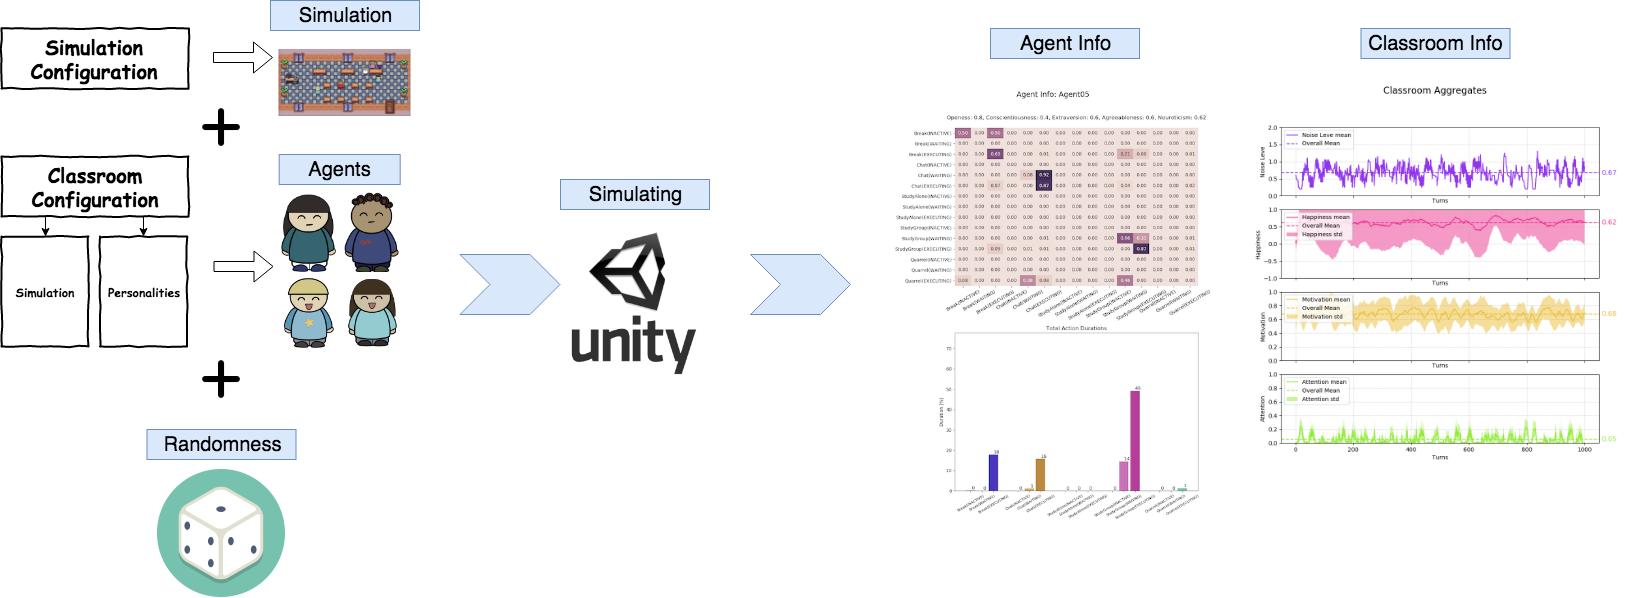
\includegraphics[width=550pt]{Simulation-Overview}
        \caption{Simulation Overview}
        \label{SimulationOverview}
    \end{minipage}    
    }%
\end{figure}

\textit{Simulation} is the first step of the analysis, answering the question how
a specific classroom of agents behaves.

The simulation program takes three input arguments. The simulation config,
is defining all simulation relevant parameters that govern how the simulation mechanism
works, the classroom configuration that defines the psychological profile of students,
and a random seed that is used to initialize the random number generator used during
the simulation.

Examples files of the simulation config and classroom config can be found as part of
the appendix (see \ref{ApxSimulationConfig} and \ref{ApxClassroomProfile}).

The classroom configuration must contain a set of Personality Types and the number
of students of each type. When the simulation is run, a classroom is dynamically
generated and filled with agents as defined.

The python analysis scripts for the simulation will process the CSV file produced
after the simulation is completed and will generate a set of figures containing information
about each individual agent, the classroom as a group and a new CSV file that contains
aggregated information.

\subsection{Agent Info}
One of the results of the simulation step is the \textbf{Agent Info} figure (see \ref{AgentInfo} showing
three different agent infos) that is generated for each agent, and contains information
about the distribution and transitions between different behaviors performed by the agent.
This figure is used to study how a specific instance of a psychological type behaves
in the given classroom. One can observe how much of the overall time an Agent
spends Studying alone or how long on average a single study session lasts.

\bb

It is interesting to observe the different patterns with which the personality traits
affect the behavior distribution of the individual agents. One could for example
observe that agents high on conscientiousness, on average have longer
learning sessions than agents that are low on conscientiousness.

\begin{figure}[H]
    \label{AgentInfo}
    \hspace*{-2.0\leftmargin}
    \makebox[\paperwidth][c]{%
        \begin{minipage}[t]{400pt}
            \centering
            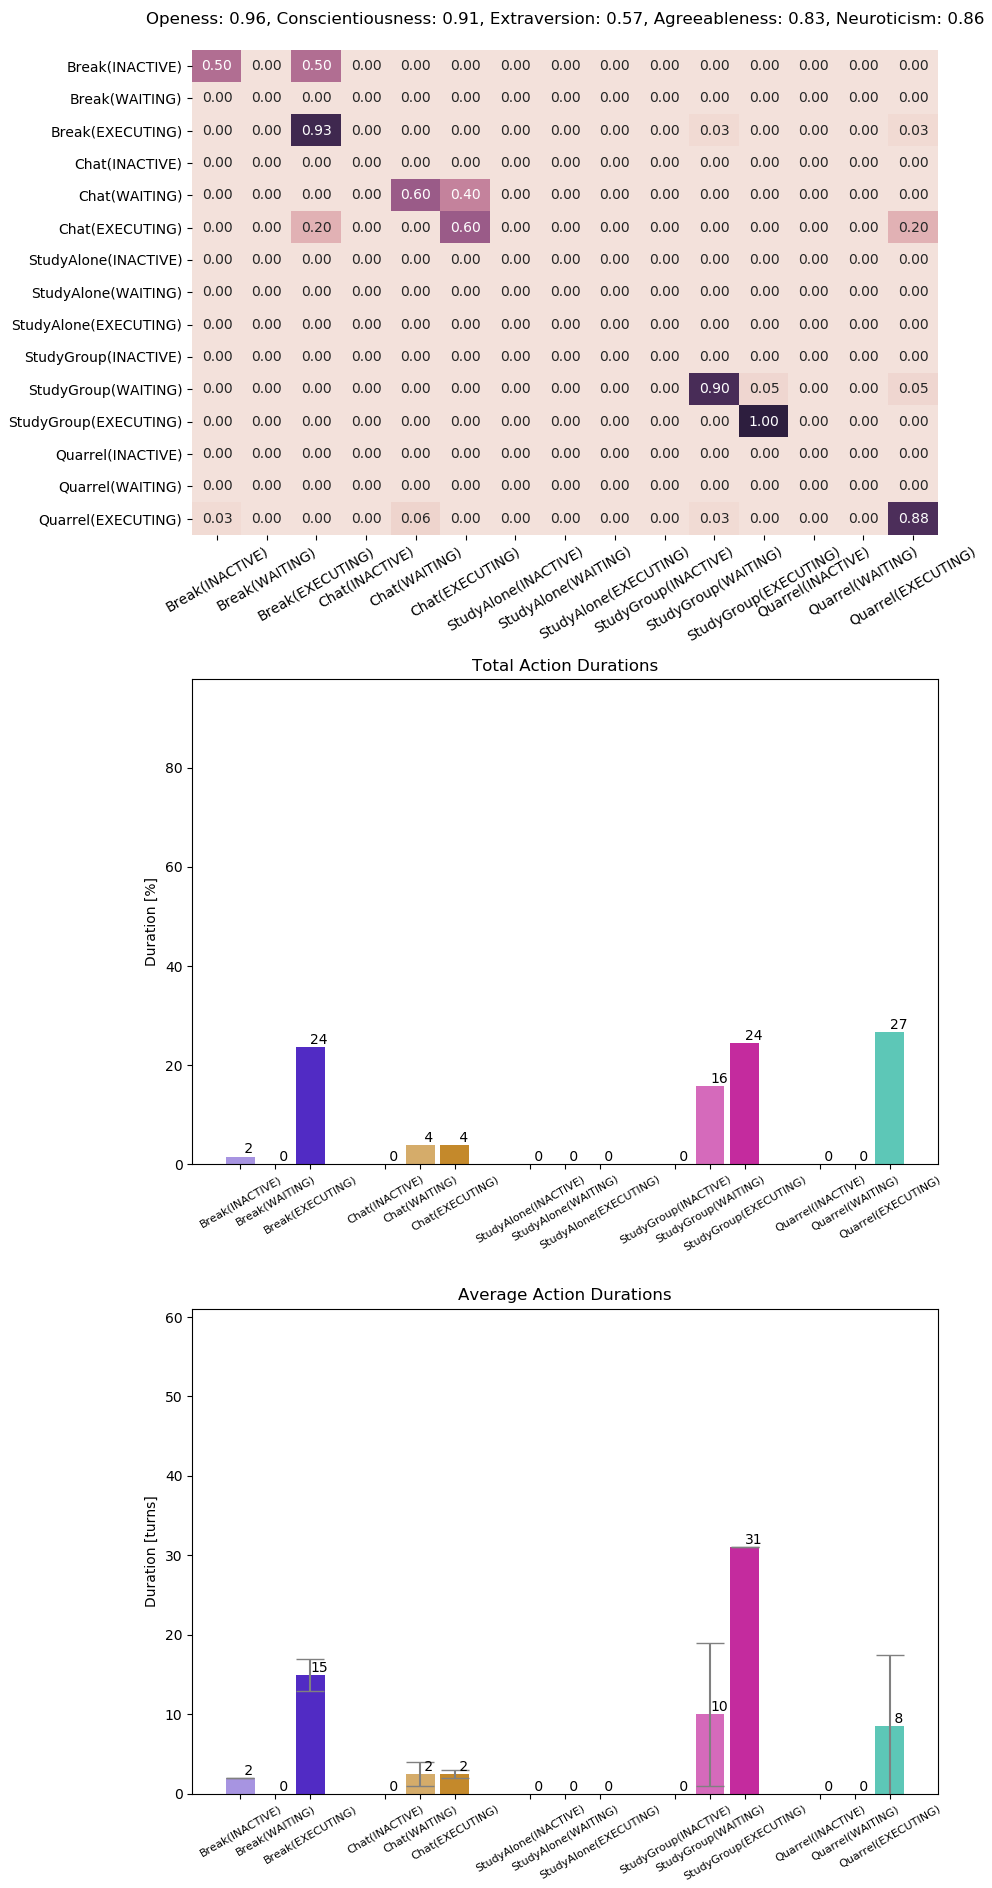
\includegraphics[width=330pt]{AgentInfo1}
            \caption{Agent Info}
        \end{minipage}
    }%
\end{figure}

\subsection{Classroom Aggregates}
The second result produced by the simulation analysis is a figure showing classroom
aggregated features over time (see figure \ref{ClassroomAggregates} as an example).
This figures contains information like the aggregated noise, average happiness,
motivation and attention of a class, in addition to information about how many of
the students are studying or quarreling at a specific moment during the simulation.

This kind of figure is useful to study how personality profiles effect the group
as a whole, and can be used to search for emerging social phenomena.

\begin{figure}[]
    \label{ClassroomAggregates}
    \hspace*{-1.0\leftmargin}
    \makebox[\paperwidth][l]{%
    \begin{minipage}[t]{10cm}
        \centering
        \includegraphics[width=450pt]{ClassroomAggregates}
        \caption{Classroom Aggregates}
    \end{minipage}    
    }%
\end{figure}


%%%%%%%%%%%%%%%%%%%%%%%%%%%%%%%%%%%%%%%%%%%%%%%%%%%%%%%%%%%%%%%%%%%%%%%%%%%%%%%%

\section{Experiment}
The experiment is the second phase of the data analysis pipeline and is focused
on evaluating the variance between simulations of the same classroom configuration.

\begin{figure}[H]
    \makebox[\textwidth][l]{%
    \begin{minipage}[t]{10cm}
        \centering
        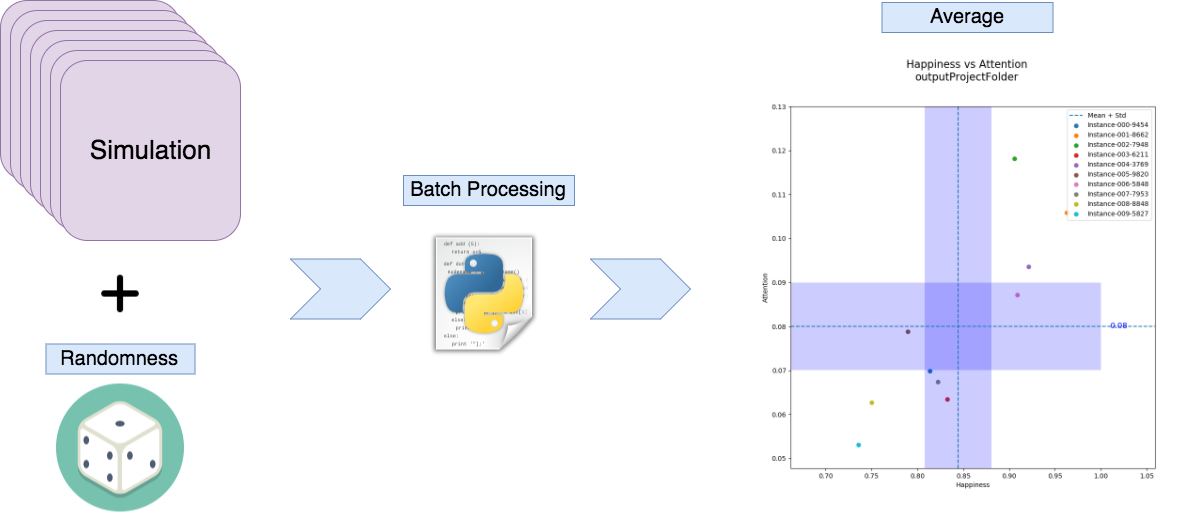
\includegraphics[width=400pt]{Experiment-Overview}
        \caption{Experiment Overview}
        \label{ExperimentOverview}
    \end{minipage}    
    }%
\end{figure}

In order to have a statistical description of the simulation results, one has to
run multiple instances of the same simulation (identical simulation  and classroom
configs) but different seed values for the random number generator used during the simulation.

There are several random elements in the simulation. Depending on the classroom
configuration, agent personality can be partially randomized. The actions selection
process has a random element, and agent interactions are effected by the output of
a random number generator.

\bb

The result of the experiment phase is a single \textbf{HA-Plot}, named after
its axis Attention and Happiness. The plot shows a a single point for each simulation
instance, with its position being based on the average attention and happiness of
the corresponding classroom over the complete simulation.

In addition the average happiness and attention over all instances is
indicated with two solid lines, and the corresponding standard deviation with
semi transparent bars.

The plot helps to identify the spread between different instances of the simulation, and
could be used to detect outliers and estimate the stability of a specific classroom
configuration.

In addition to the HA-Plot a CSV file is generated that contains the average
happiness and attention for each agent and classroom for all simulation instances.
This dataset is the numeric equivalent to the generated HA-Plot.

%%%%%%%%%%%%%%%%%%%%%%%%%%%%%%%%%%%%%%%%%%%%%%%%%%%%%%%%%%%%%%%%%%%%%%%%%%%%%%%%

\section{Study}
The last step in the data analysis pipeline is focused on comparing different classroom
profiles.

In this phase the CSV generated during the Experiment phase is analyzed to
generate a HA-Plot that contains one ellipse for each classroom profile simulated.
The center of the ellipse is put to the overall mean of attention and happiness
of the corresponding set of instances of the same classroom profile, indicating its standard
deviation by the shape of the ellipse.

This plot gives an visual overview of the effect the different personality profiles
have compared to each other, and can be used to study the strength and direction of
change one profile has compared to another.

\begin{figure}[H]
    \makebox[\textwidth][l]{%
    \begin{minipage}[t]{10cm}
        \centering
        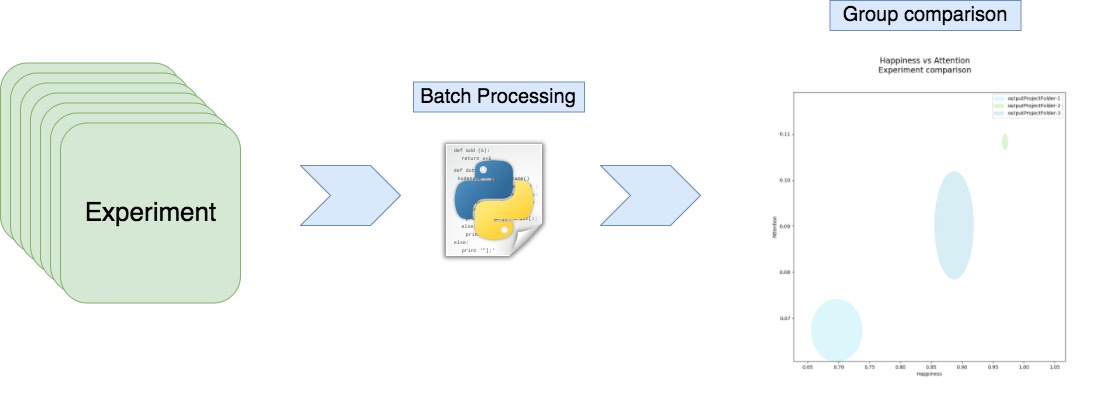
\includegraphics[width=400pt]{Study-Overview}
        \caption{Study Overview}
        \label{StudyOverview}
    \end{minipage}    
    }%
\end{figure}


\chapter{Study and Results}
In this chapter we will present the study that has been performed and the results
generated using our simulation.

\section{ADHD and Personality Traits}
A recent study \cite{Polanczyk2015} shows that the world wide prevalence
for anxiety disorders within children and adolescents to be around 6.5\%, and 
Attention-deficit hyperactivity disorder \textbf{(ADHD)}\cite{Barkley1997} being one
of the most common childhood behavioral disorder, ranging between 5\% and 10\% \cite{Sayal2018}.

\bb

Because of the high prevalence of anxiety disorders in the general population,
and the availability of studies correlating ADHD with personality traits, we
decided to study the effect of children with personality profiles that match those
of ADHD patients on the class as a whole.

\bb

The primary reference for how ADHD symptoms relate to personality traits, we took
from \cite{Nigg2002}, where the authors write

\textit{\dots our findings for the two major symptom domains suggest the following
conclusion: overall ADHD symptoms are related to low Conscientiousness, low Agreeableness, and high Neuroticism.}

\section{Study Description}
The study we performed had the objective to simulate how an increasing number of
students with ADHD symptoms would affect the group dynamics. This was achieved by
the following steps.

\begin{itemize}
    \item We defined three types of students (\textit{ADHD, Normal, Ambitious})
    \item Created several classroom profiles varying the ratio of the different student types present
    \item Run a Simulation study comparing the classroom profiles to each other
\end{itemize}

\subsection{Student Types}
The student types chosen have been inspired by the literature, whereby we 
took defined a ADHD student using results from \cite{Nigg2002}, a normal type using
\cite{Srivastava2003} and Ambitious students from \cite{Asendorpf2003}.

At this point it is worth to note that the defined student types are prototypical in nature.
There exists no \textit{normal} nor \textit{ADHD} personality trait type. The Big-Five
model is a continuos scale in all five dimensions. The different personality types
have been defined as a shorthand to simplify the analysis of results and highlight
the divergence between groups.

The concrete personality profiles used for each type are found in table \ref{StudenTypesTable}

\begin{table}[h!]
    \centering
    \begin{tabular}{|l|c|c|c|c|c|} 
        \hline
        \textbf{Student Type} & \textbf{O} & \textbf{C} & \textbf{E} & \textbf{A} & \textbf{N} \\
        \hline
        \hline
        ADHD & RND & 0.20 & RND & 0.20 & 0.80 \\
        \hline
        Normal & 0.75 & 0.60 & 0.55 & 0.65 & 0.50 \\
        \hline
        Ambitious & 0.80 & 0.80 & RND & 0.80 & 0.20 \\
        \hline
        Random & RND & RND & RND & RND & RND \\
        \hline
    \end{tabular}
    \caption{Table with Student types composition groups}
    \small RND indicates a random value from a uniform distribution between [0, 1]
    \label{StudenTypesTable}
\end{table}

\subsection{Groups}
Based on the student types we created various classrooms that where compared to
each other. Each group consisted of 30 students, varying the \% of each Student
type per group (see table \ref{GroupTable}).

The ratio of ADHD students is very high and does not correspond directly to
empirical findings (see \cite{Sayal2018} who estimates ratios to be between 5-10\%).
We have chosen those high values because ADHD is no black or white form of psychological
disorder, but rather a spectrum that can vary strongly in its intensity and persons behavior.
Similar to the student types, the different groups have been defined to exemplify
tendencies and highlight differences.

In addition the group 'Random' serves as a form of estimation how strong the simulation
output is affected by the classroom profile.

\begin{table}[h!]
    \centering
    \begin{tabular}{|l|c|c|c|c|} 
        \hline
        \textbf{Group} & \textbf{ADHD} & \textbf{Normal} & \textbf{Ambitious} &  \textbf{Random} \\
        \hline
        \hline
        ADHD-Low & 7\% & 93\% & 0\% & 0\% \\
        \hline
        ADHD-Medium & 17\% & 83\% & 0\% & 0\% \\
        \hline
        ADHD-High & 33\% & 66\% & 0\% & 0\% \\
        \hline
        ADHD-VeryHigh & 50\% & 50\% & 0\% & 0\% \\
        \hline
        ADHD-None & 0\% & 100\% & 0\% & 0\% \\
        \hline
        ADHD-None-Ambitious & 0\% & 50\% & 50\% & 0\% \\
        \hline
        ADHD-Low-Ambitious & 7\% & 46\% & 46\% & 0\% \\
        \hline
        ADHD-Medium-Ambitious & 20\% & 40\% & 40\% & 0\%\\
        \hline
        ADHD-VeryHigh-Ambitious & 50\% & 0\% & 50\% & 0\%\\
        \hline
        Random & 0\% & 0\% & 0\% & 100\% \\
        \hline
    \end{tabular}
    \caption{Groups composition studied}
    \small RND indicates a random value from a uniform distribution between [0, 1]
    \label{GroupTable}
\end{table}

\section{Results}
We have been simulation each of the groups defined above using 5 replicates, initiated
with different seed values.

The HA-Plot is generated by the last step of the Data Analysis is shown in figure \ref{StudyResults}.

\begin{figure}[H]
    \caption{HA-Plot comparing the different classroom configurations}
    \label{StudyResults}
    \makebox[\textwidth][l]{%
    \begin{minipage}[t]{500pt}
        \centering
        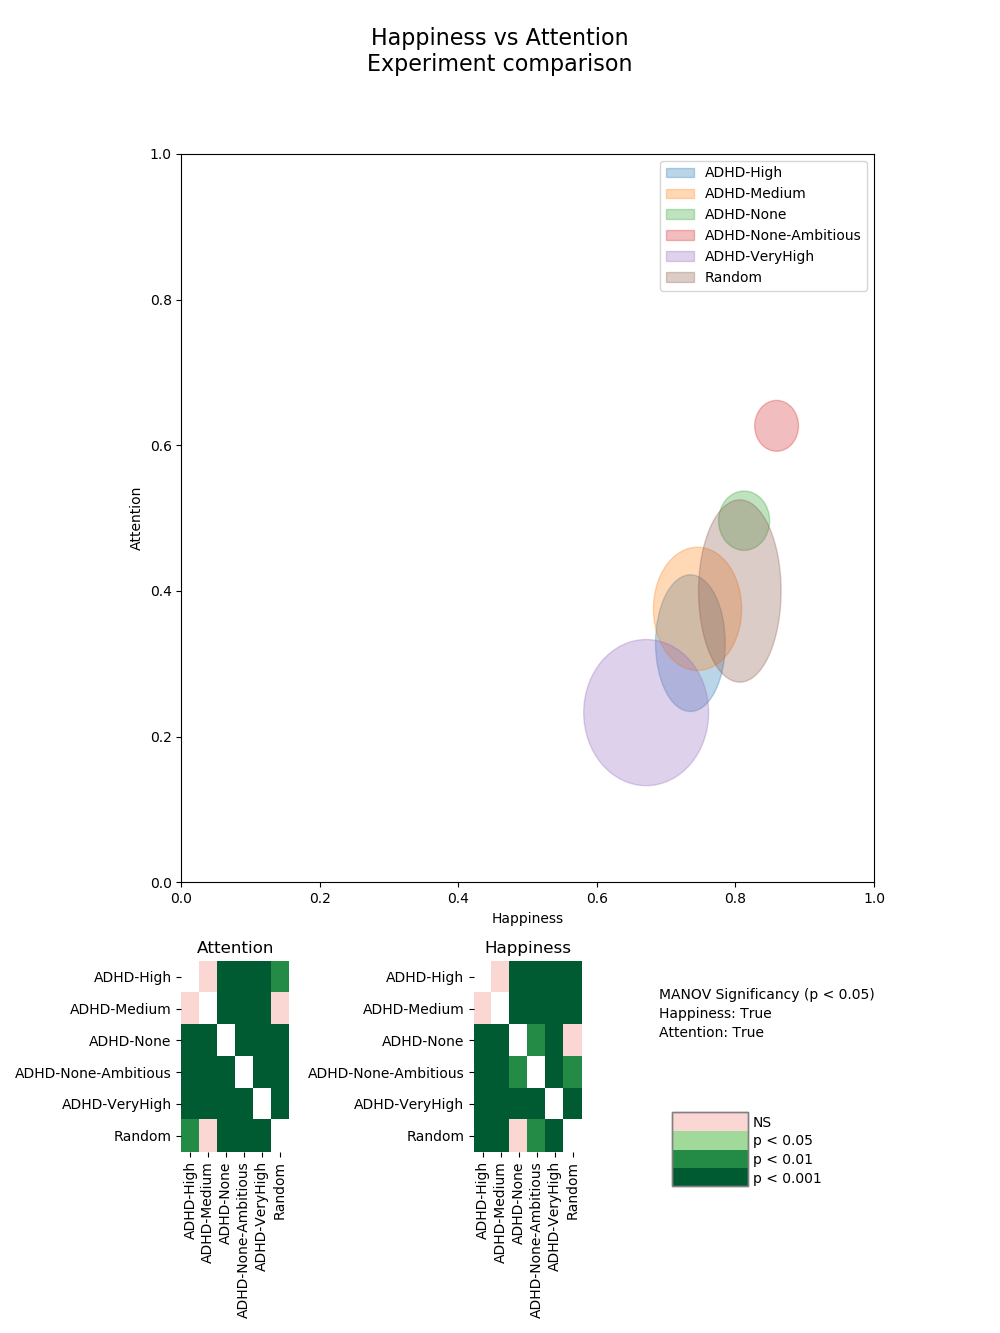
\includegraphics[width=400pt]{results/HAPlot}
    \end{minipage}    
    }%
\end{figure}

Classrooms with ADHD students had a strong effect in all groups. The general
tendency seems to be that the higher the ratio of ADHD students, less happy and
attentive the class as a whole becomes. The ambitious students on the other
side cause the exact reverse effect, increasing happiness and attention.

\subsection{ADHD Effect}
Given this dynamic, specially the groups containing a mixture of ADHD and
ambitious students is interesting. Comparing the groups \textit{ADHD-Low-Ambitious},
\textit{ADHD-Medium-Ambitious} and \textit{ADHD-VeryHigh-Ambitious} show that ADHD
type students have a far stronger effect than their ambitious counterparts.

\bb

This effect is most visible in the \textit{ADHD-Low-Ambitious} group, in which only
very few ADHD students, reduce mean happiness and attention compared to the \textit{ADHD-None}
group despite the presence of many more ambitious students.

\bb

\subsubsection{ADHD and Personality traits}
To investigate this further, we have calculated the correlation between student personality
traits and happiness, attention and conformity. The correlation matrix is part
of the HA-Plot of the final result \ref{StudyResults}. In addition we have calculated
two more correlation matrices, that contain all ADHD classrooms in one matrix, and
all None ADHD classes in the other (see figure \ref{CorrleationComparison}).

\bb

It appears that for None-ADHD Classrooms, the different personality traits are equally
correlated with the mean happiness and attention of the students. For the ADHD
classrooms on the other side there is a strong correlation for some of them, but not
for others. Happiness and Attention correlates strongly with Conscientiousness, Agreeableness
and Neuroticism; which by the way are the main personality traits for the ADHD student
type. This strong correlation between the key ADHD personality traits and the HA
axis explain the direction of the effect.

\bb

Concerning the strength of the effect, it is interesting to look at the HA-Plots
showing the individual agents of a single simulation Instance. Comparing the classroom
configurations \textit{ADHD-Low-Ambitious}, \textit{ADHD-Medium-Ambitious} and
\textit{ADHD-VeryHigh-Ambitious} contained in the \ref{AppendixChapter}, one can
see clearly that there are two clusters of agents. The ADHD agents in the lower
left and the None-ADHD agents in the upper right region of the plot.
As the ratio of ADHD students increases, the None-ADHD cluster is shifting
towards the lower left (less happy, less attention), while the ADHD cluster remains
where it was.

\bb

It appears that the ADHD students cause a strong shift in behavior of the None-ADHD
agents, without altering or adapting their own.

\begin{figure}[]
    \centering
    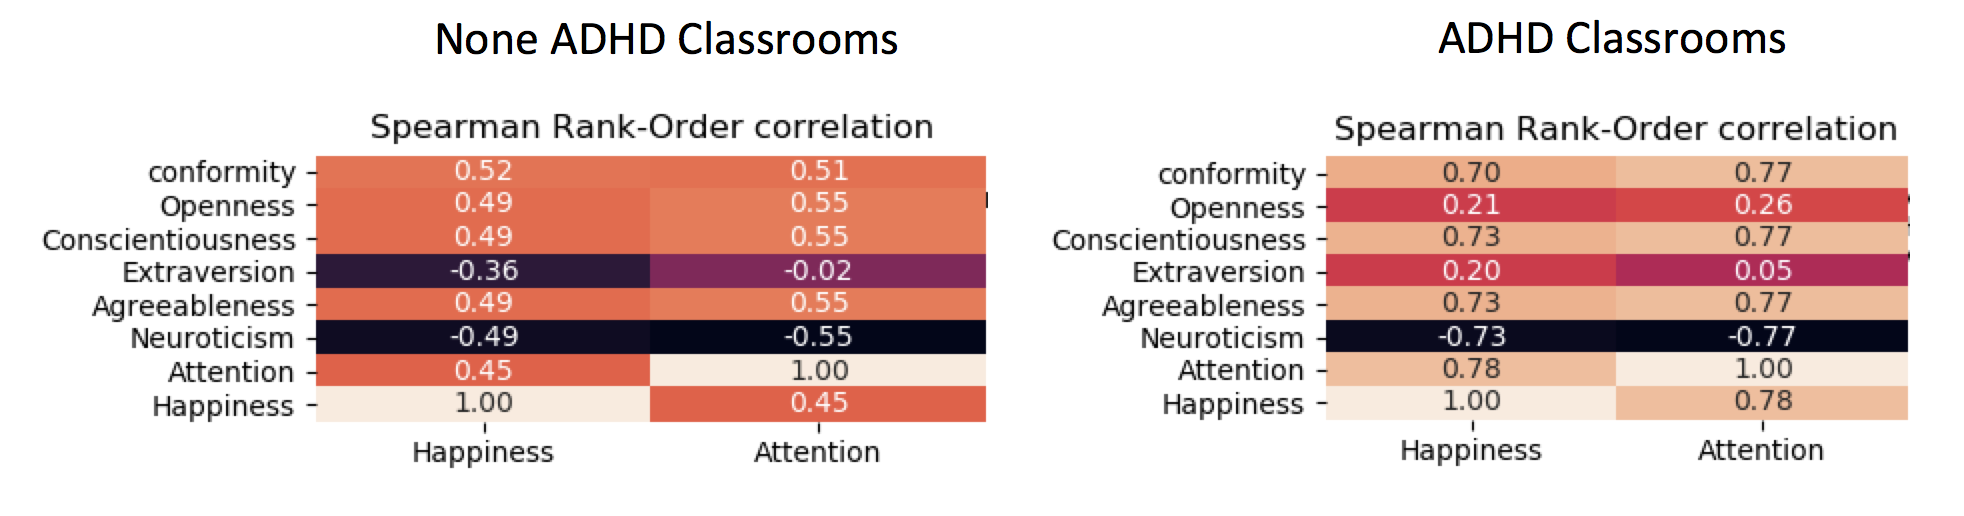
\includegraphics[width=400pt]{results/CorrelationComparison}
    \caption{Comparing change in correlation between ADHD and None-ADHD Classrooms}
    \label{CorrleationComparison}
\end{figure}

\subsection{Classroom riots}
Finally we want to shortly compare the classroom aggregate plots of the classroom
configurations \textit{ADHD-High}, \textit{ADHD-None},  \textit{ADHD-None-Ambitious} and
\textit{ADHD-Low-Ambitious}.

\bb

It appears that the \textit{ADHD-High} class compared to the \textit{ADHD-None}
has less regular cycles of studying and breaks, while increasing the number of
class wide episodes of quarrel (i.e. classroom riots). Those class wide quarrels
are an interesting phenomena that can be observed in all classroom configurations. 

\bb

Comparing the effect of few ADHD students in an ambitious classroom (groups
\textit{ADHD-None-Ambitious} and \textit{ADHD-Low-Ambitious}) one immediately
notices the increased number of class wide quarrels. In addition it is interesting
to see that the \textit{ADHD-None-Ambitious} has a tendency to be in one of
two extreme cases of either none or almost everyone quarreling. 


\chapter{Conclusion and outlook}
In this chapter we will draw our final conclusions, including an outlook on
possible directions to continue and improve the work done so far.

\section{Conclusion}
As part of the thesis we have developed a multi-agent model that is simulating a virtual classroom.

We have devised a Agent Logic that is based on the established Big-Five Personality
Trait model and that produces agent behavior consistent with empirical studies.

We have developed a data analysis pipeline that makes it possible to efficiently
run multiple simulations in a batch mode, enabling a statistical analysis of the
simulation results.

We chose to compare how students with prototypical ADHD personality traits affect
the classroom dynamics, and therefore defined multiple classrooms varying in 
ratio between none to a high number of ADHD students.

We found that students have a very strong effect on the average happiness and attention
of the class. It appears that ADHD students affect the behavior of None-ADHD Students
without changing their won. In addition we found that even a low number of
ADHD students cause more frequent riots, specially in classrooms with very
ambitious students.

The simulation software, the data analysis scripts and all content presented in this
thesis is available freely under the MIT License from the github repository
\href{https://github.com/mapa17/breakfastclub}{https://github.com/mapa17/breakfastclub}.

\section{Outlook}
As mentioned shortly in the chapter on Objectives some initial objectives had to
be dropped during the development of the thesis in order to stay within the available
time frame.

The following is a list of possible improvements, as well as ideas for follow up projects.

\begin{itemize}
    \item \textbf{Improve classroom analysis:}
    The HA-Plot for different classroom configurations is a very concise representation
    of multiple instances of the same classroom configuration. Many of the temporal
    dynamics shown in the classroom aggregate plot are not visible in the HA-Plot.
    In addition there is no direct way to compare classroom aggregate plots.

    \bb

    Methods from Time series analysis could be used to extract information about
    the signal dynamics (like periodicity, entropy, moments, ...) in order to compare
    instances of the same classroom configuration or between different configurations.

    \bb

    It would be particularly useful extract a \textit{typical} classroom aggregate
    showing the classroom dynamics for an configuration and not only an instance.
    \item \textbf{Interactive Simulation:} 
    On way to extend how the simulation can be used, is to make the simulation
    interactive. Doing so would provide the user with the option to force agents
    to perform certain actions, expulse students from the classroom, call for silence
    or similar interactions. This would make it possible to develop a teacher training 
    program, based on the simulator, similar to commercial solutions like TLE TeachLive
    \cite{Dieker2017} or simSchool \cite{Badiee2015} but open source and with
    agent behavior that is based on a psychological model.
    
    \bb
    
    In order to support learning and provide a novel visualization of the effect
    of user interaction with the simulation we envisioned a system that is able to track
    the effect of each user interaction onto the final result of the simulation.
    This could be achieved by creating a clone of the running simulation when ever
    the user is performing an action. That clone instance would continue until the 
    end of the simulation unperturbed, and could be compared to the all other clones
    generated in the same way. This would make it possible to evaluate the effect
    of each user interaction onto the final result of the simulation, and visualize it
    as a trace instead of a dot in the HA-Plot.

    \item \textbf{Reinforcement trained teacher:} At the moment the simulation
    is consisting of students that behave like an autonomous study group.
    With the teacher interactions described in the previously, one could train a
    virtual teacher using reinforcement learning (RL) with
    the objective to maximize happiness and attention of the class.
    
    \bb

    As there is a fast amount of literature on different teaching methodologies,
    it would be interesting to study if the RL trained teacher applies any of the known
    methodologies or applies new ones. Another interesting aspect would be to study the
    effect different classroom profiles have on the trained teacher, with other
    word, how different classroom profiles form and shape teacher behavior.

    \item \textbf{Screening of classroom profiles:} One obvious extension based
    on the batch processing capabilities of the simulation is to perform a kind
    of screening studying. One would systematically evaluate a high number of personality
    profiles, similar to screening studies in Bioinformatics, comparing thousands
    of combination in order to find interesting tipping points, extremes and curious
    singularities.

    \item \textbf{Dominance hierarchy:} The current simulation when calculating
    the peer pressure on a individual agent is modeling a flat social hierarchy.
    One could extend this to a more realistic Dominance Hierarchy, giving different
    agents different weights in controlling the classroom interest. Such a Dominance
    hierarchy in place one could extend its effect on other actions like chat or
    quarrel, making the outcome of interactions depend as well on the position
    of agents in the dominance hierarchy.

    \item \textbf{Learning Agents:} Because of simplicity the agents have no capability
    to learn and adapt their behavior over time. One could prevent some simple learning
    mechanisms, that would open a wide range of new questions one can study, concerning
    the dynamics of agent and group behavior over longer durations of time.
\end{itemize}

\section{Acknowledgement}
We especially want to thank Prof. Dr. Michael Kickmeier-Rust for his continuos
support and mentoring. Without him this work would have not been possible.


\chapter{Bibliography}
\bibliographystyle{ieeetr} 
\bibliography{bibliography}

\chapter{Article}
% TODO: Have to center pdf
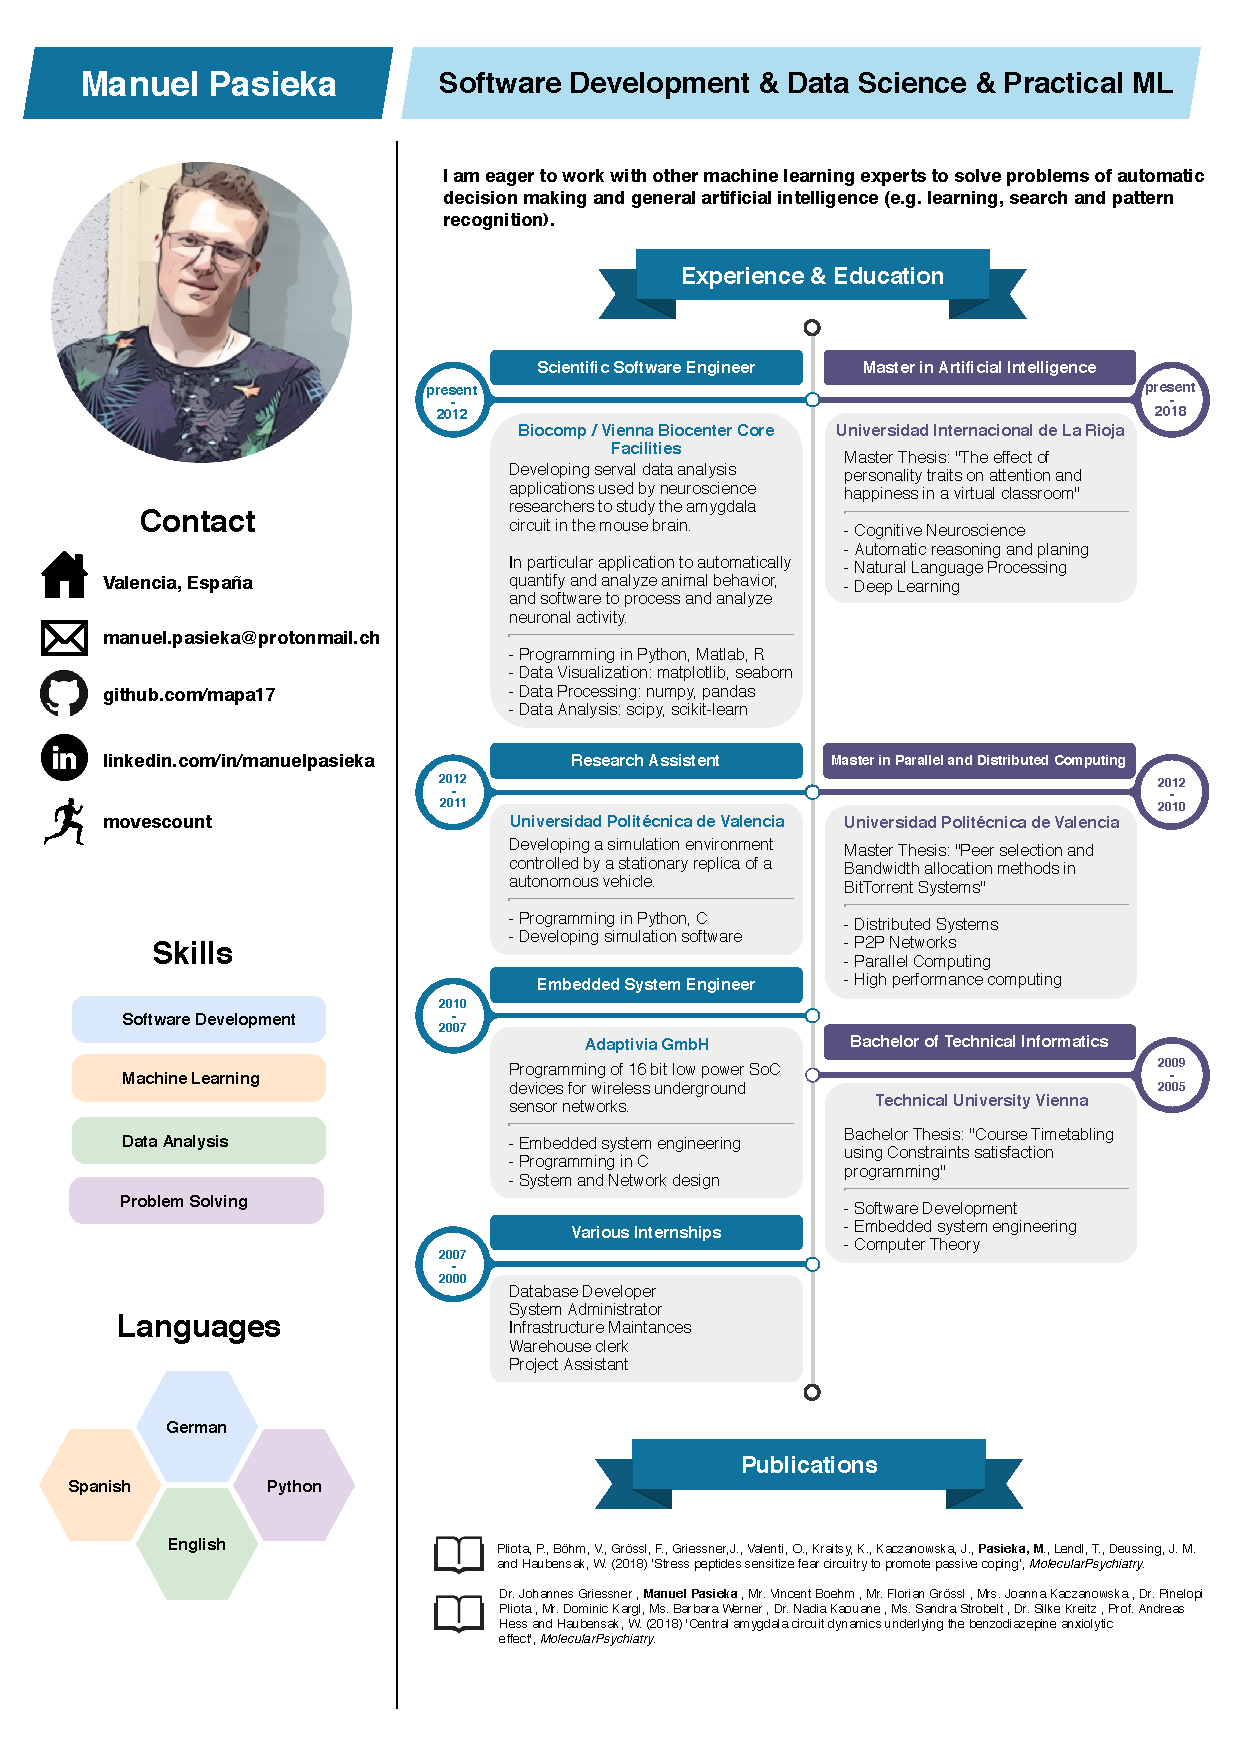
\includepdf[pages=-, fitpaper=true]{appendix/Article.pdf} 


\appendix

\chapter{Appendix}

\label{ApxSimulationConfig}
\section{Simulation Config}
\lstinputlisting[language=Python]{appendix/SimulationConfig.json}

\label{ApxClassroomProfile}
\section{Classroom Config}
\lstinputlisting[language=Python]{appendix/ClassroomConfig.json}

\label{ApxResults}

%%%%%%%%%%%%%%%%%%%%%%%%%%%%%%%%%%%%%%%%%%%%%%%%%%%%%%%%%%%%%%%%%%%%%%%%%%%%%%%%

\section{Results}

\subsection{ADHD-Low}

\begin{figure}[H]
    \centering
    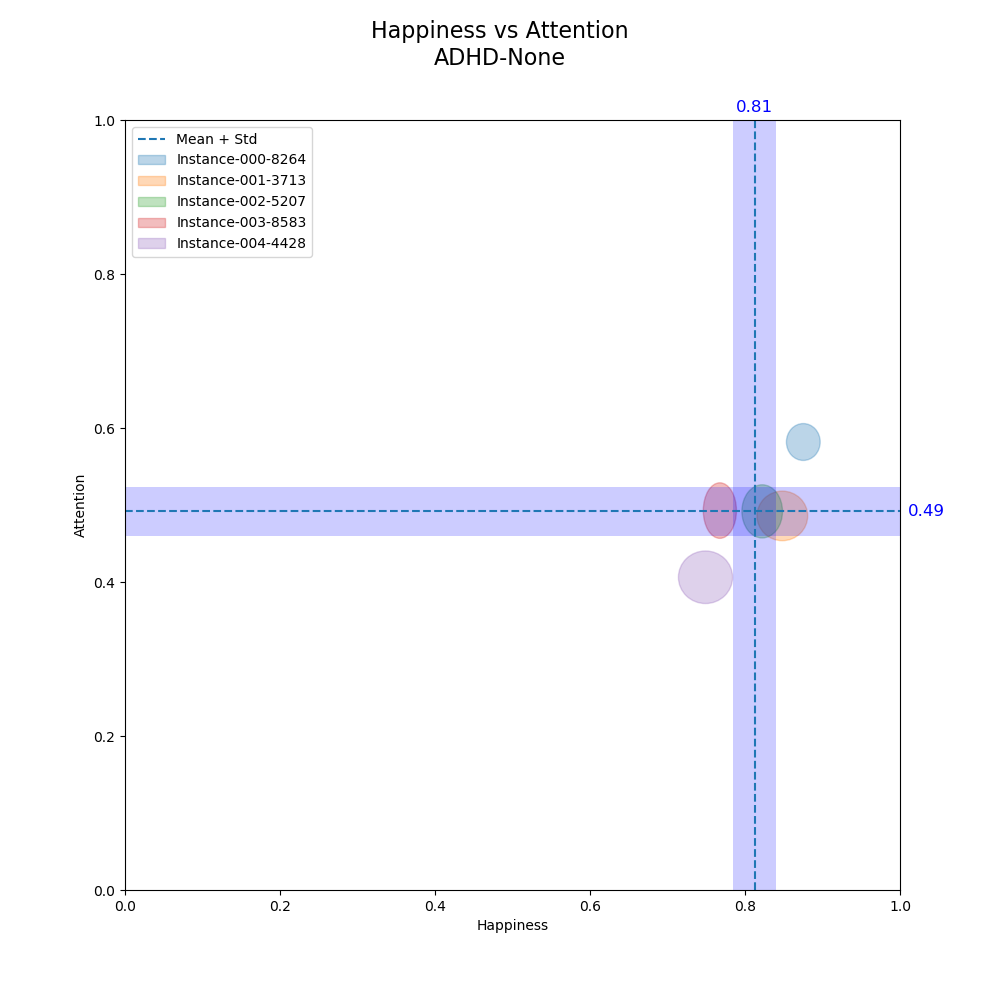
\includegraphics[width=500pt]{results/ADHD-Low/Experiment_summary-AgentStd}
    \caption{HA Plot for complete experiment}
\end{figure}

\begin{figure}[H]
    \centering
    \includegraphics[width=500pt]{results/ADHD-Low/HA-Plot}
    \caption{HA Plot for first instance}
\end{figure}

\begin{figure}[H]
    \centering
    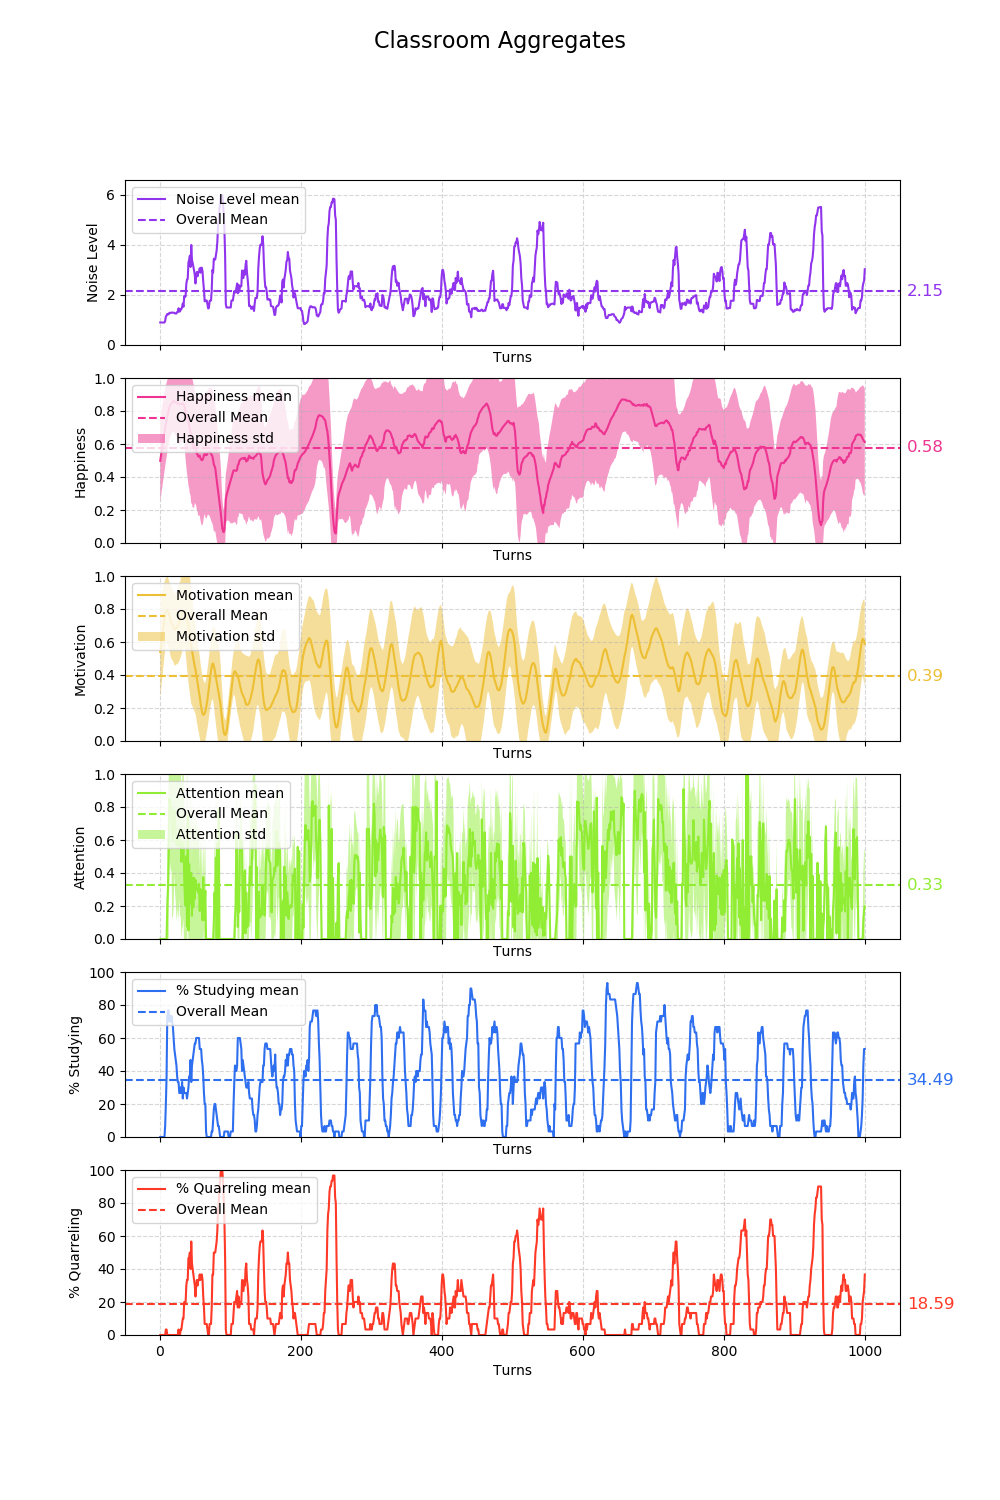
\includegraphics[width=400pt]{results/ADHD-Low/ClassroomAggregates}
    \caption{Classroom aggregates for first instance}
\end{figure}


%%%%%%%%%%%%%%%%%%%%%%%%%%%%%%%%%%%%%%%%%%%%%%%%%%%%%%%%%%%%%%%%%%%%%%%%%%%%%%%%
\subsection{ADHD-Medium}

\begin{figure}[H]
    \centering
    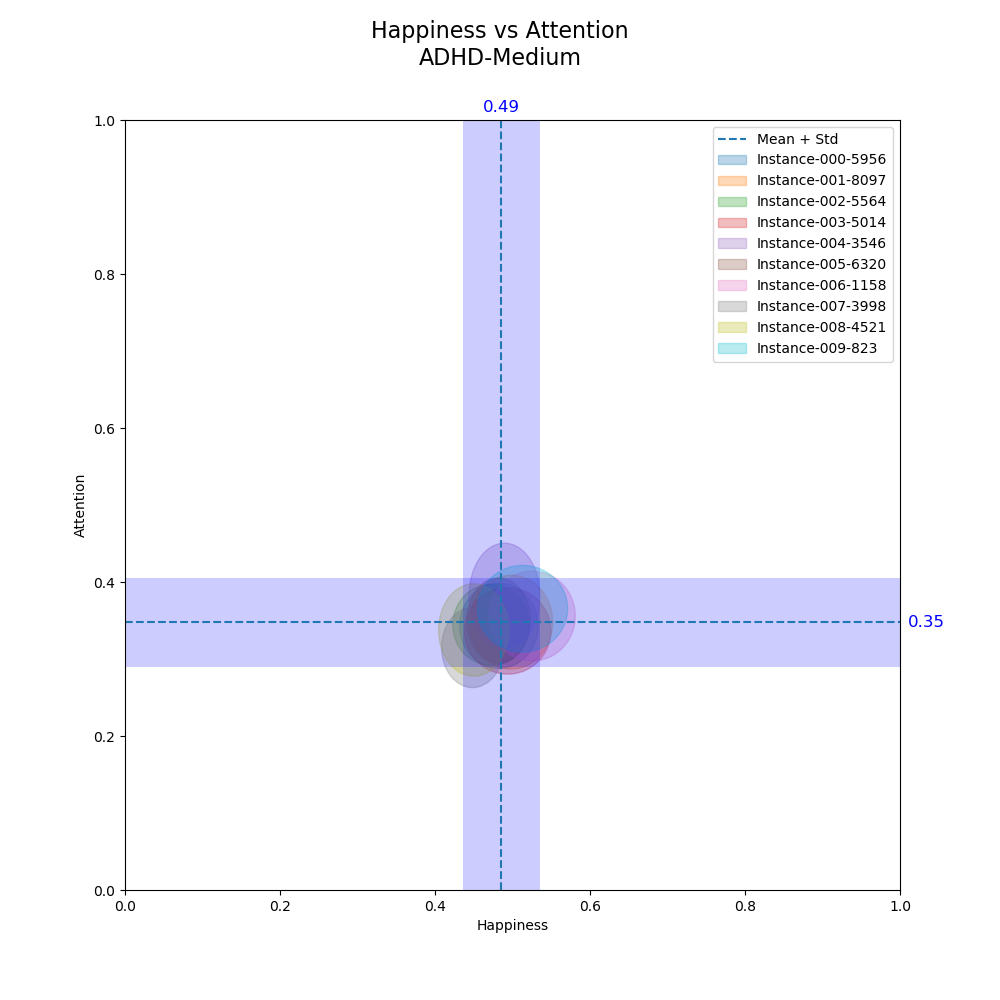
\includegraphics[width=500pt]{results/ADHD-Medium/Experiment_summary-AgentStd}
    \caption{HA Plot for complete experiment}
\end{figure}

\begin{figure}[H]
    \centering
    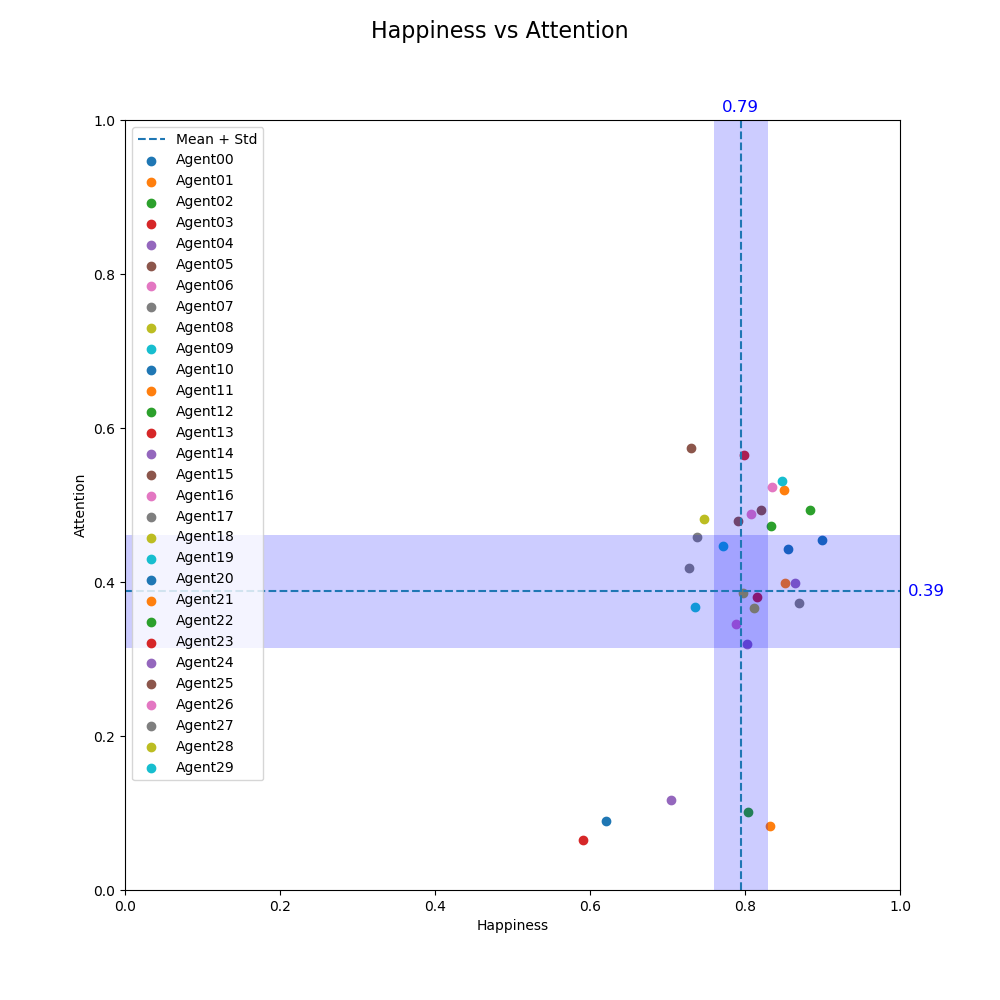
\includegraphics[width=500pt]{results/ADHD-Medium/HA-Plot}
    \caption{HA Plot for first instance}
\end{figure}

\begin{figure}[H]
    \centering
    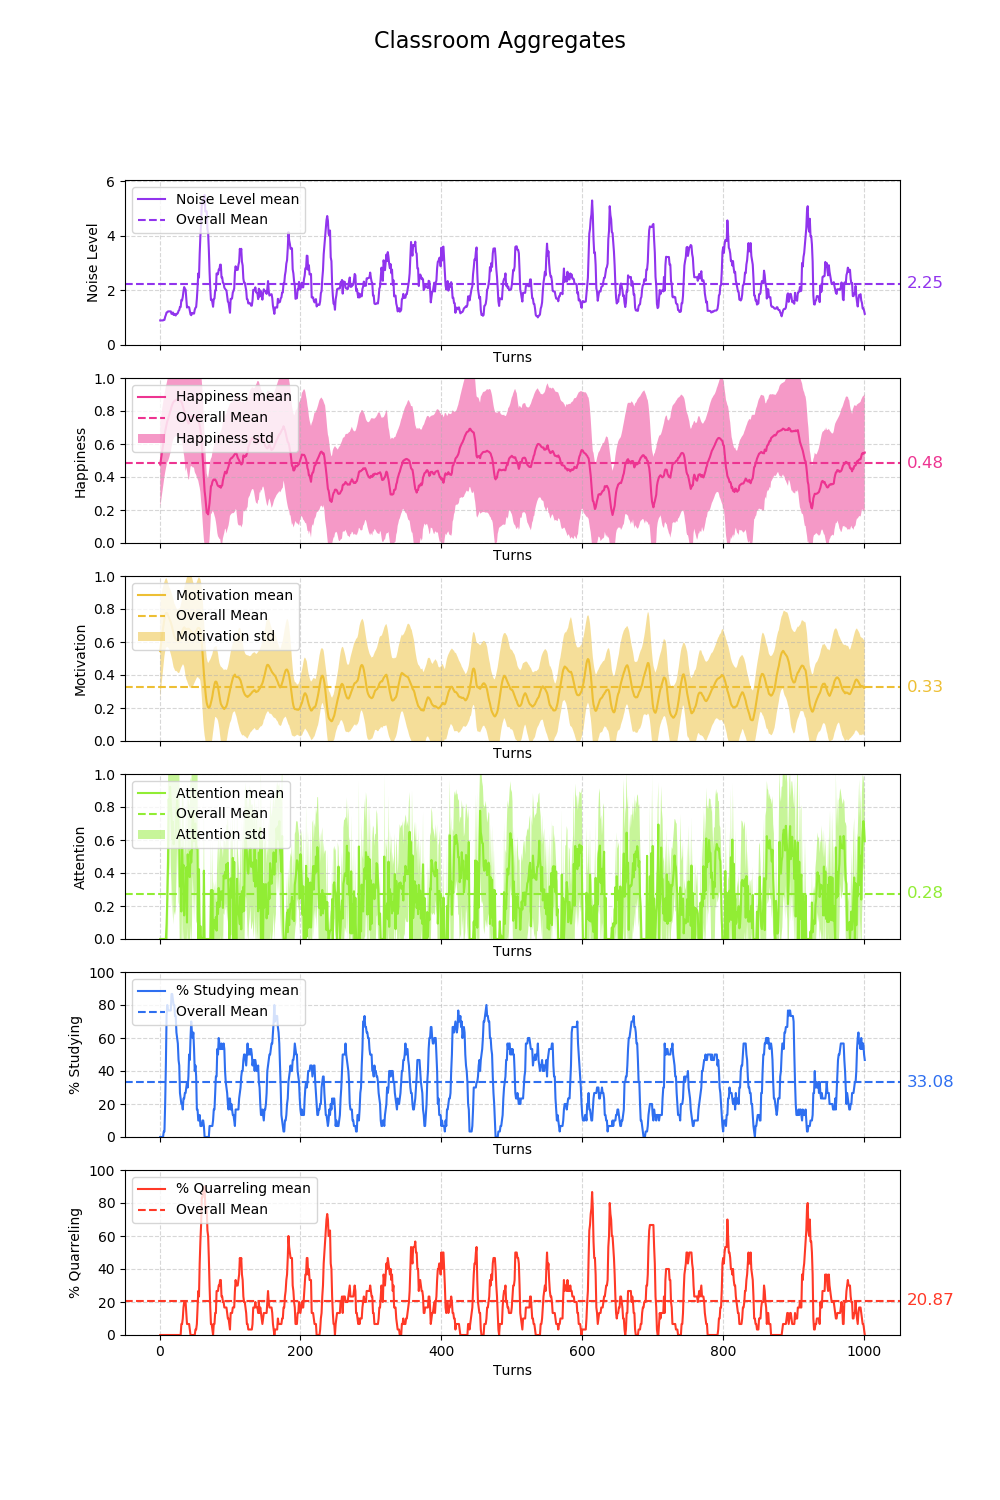
\includegraphics[width=400pt]{results/ADHD-Medium/ClassroomAggregates}
    \caption{Classroom aggregates for first instance}
\end{figure}


%%%%%%%%%%%%%%%%%%%%%%%%%%%%%%%%%%%%%%%%%%%%%%%%%%%%%%%%%%%%%%%%%%%%%%%%%%%%%%%%
\subsection{ADHD-High}

\begin{figure}[H]
    \centering
    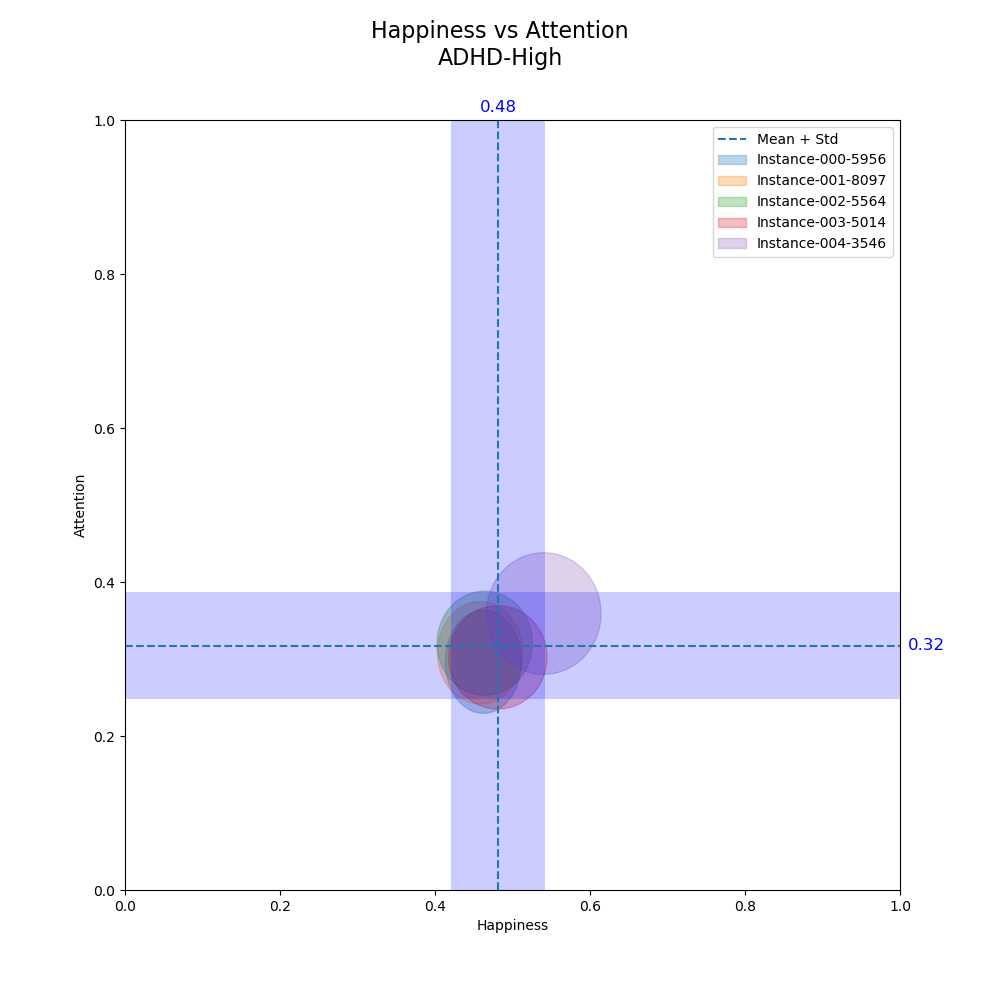
\includegraphics[width=500pt]{results/ADHD-High/Experiment_summary-AgentStd}
    \caption{HA Plot for complete experiment}
\end{figure}

\begin{figure}[H]
    \centering
    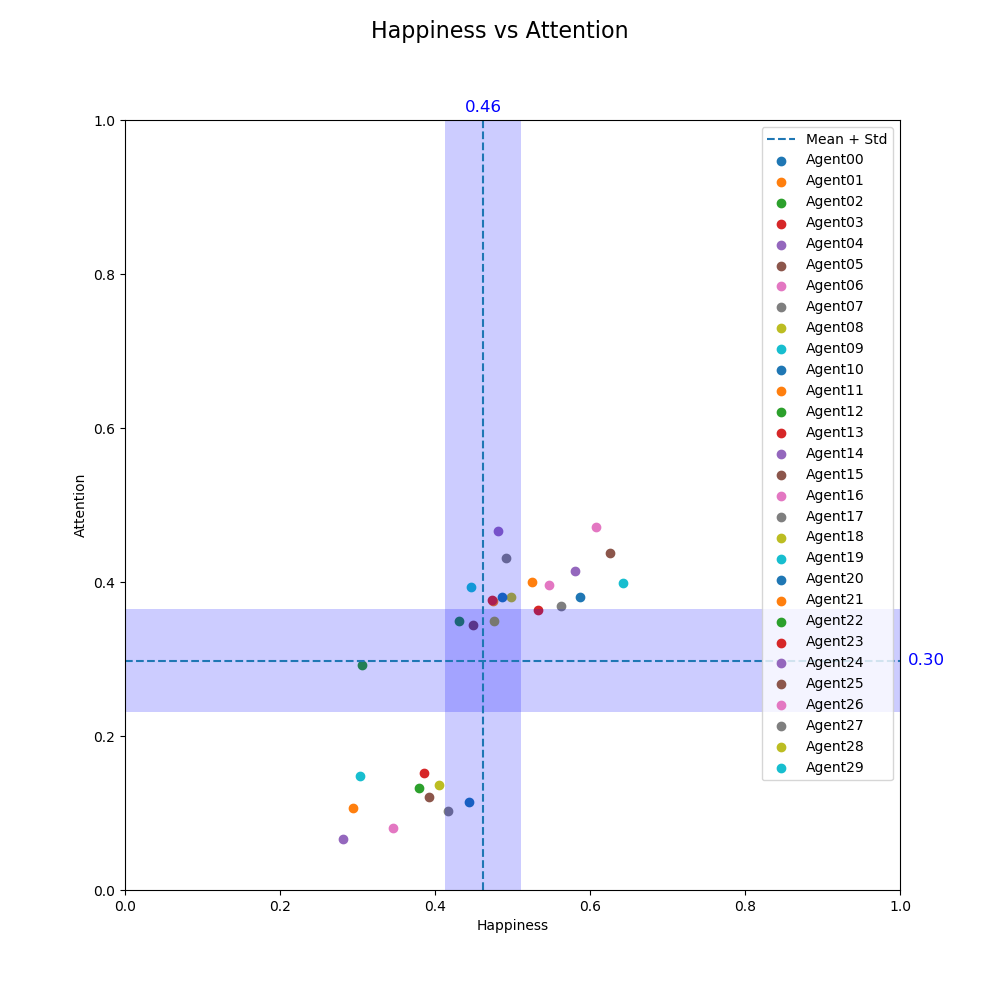
\includegraphics[width=500pt]{results/ADHD-High/HA-Plot}
    \caption{HA Plot for first instance}
\end{figure}

\begin{figure}[H]
    \centering
    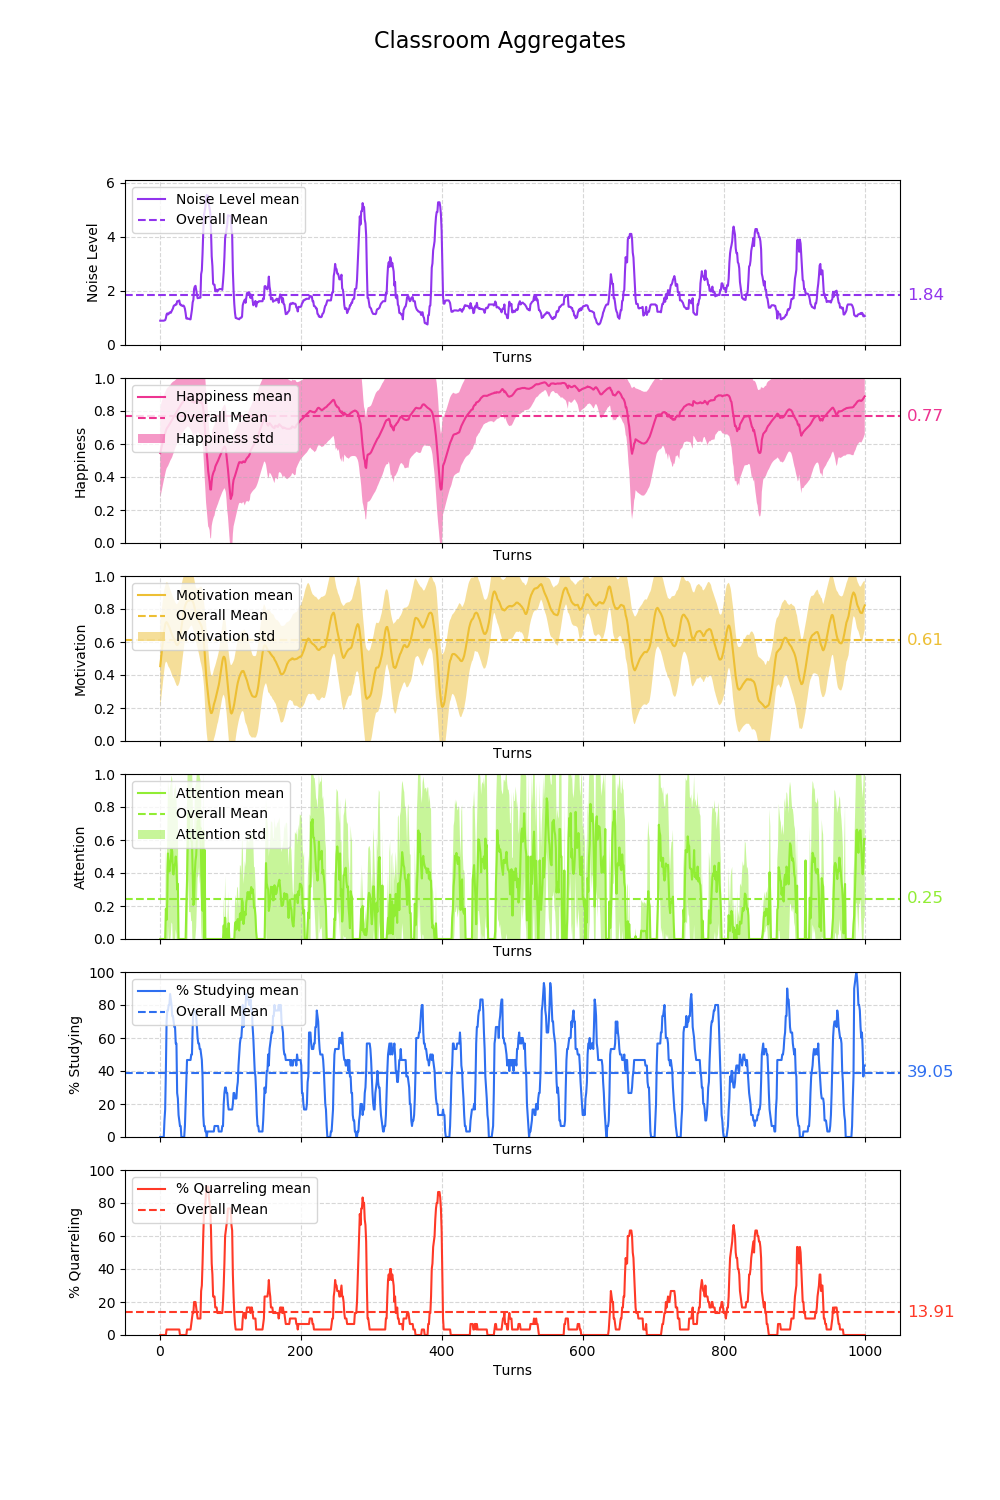
\includegraphics[width=400pt]{results/ADHD-High/ClassroomAggregates}
    \caption{Classroom aggregates for first instance}
\end{figure}


%%%%%%%%%%%%%%%%%%%%%%%%%%%%%%%%%%%%%%%%%%%%%%%%%%%%%%%%%%%%%%%%%%%%%%%%%%%%%%%%
\subsection{ADHD-VeryHigh}

\begin{figure}[H]
    \centering
    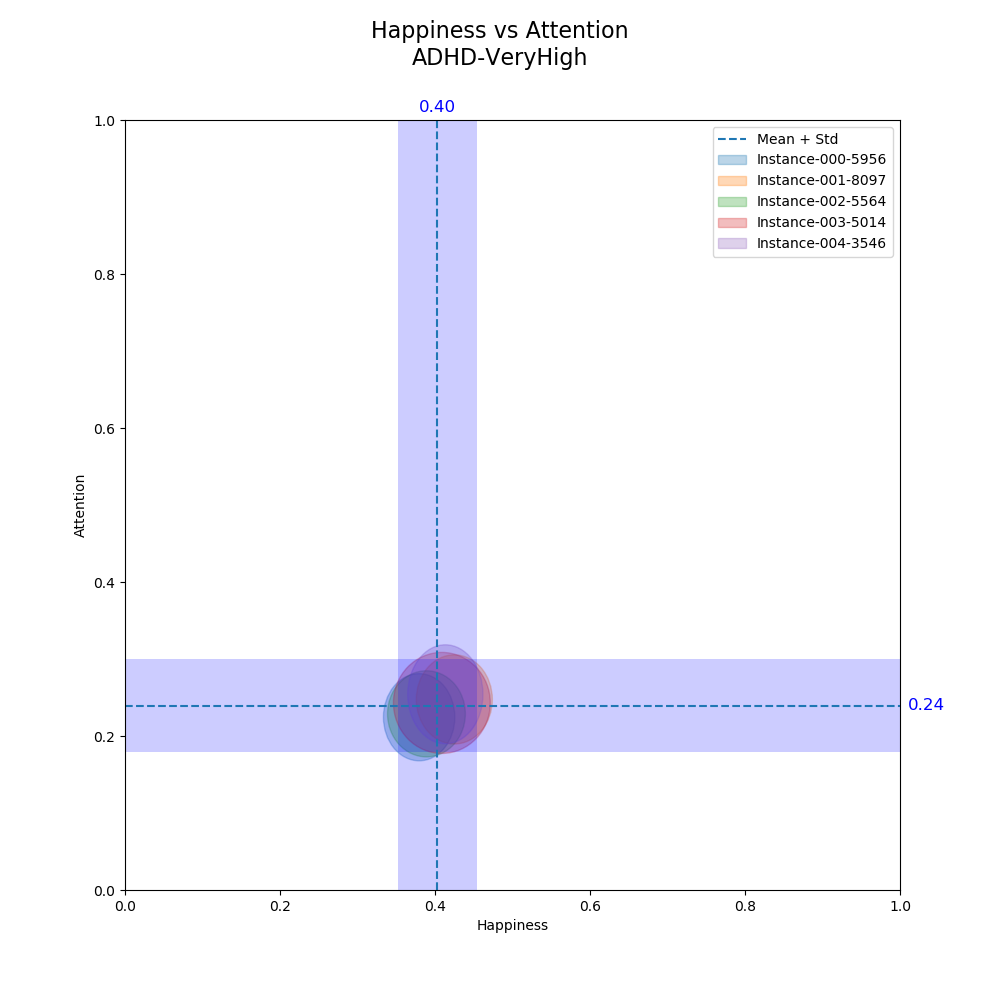
\includegraphics[width=500pt]{results/ADHD-VeryHigh/Experiment_summary-AgentStd}
    \caption{HA Plot for complete experiment}
\end{figure}

\begin{figure}[H]
    \centering
    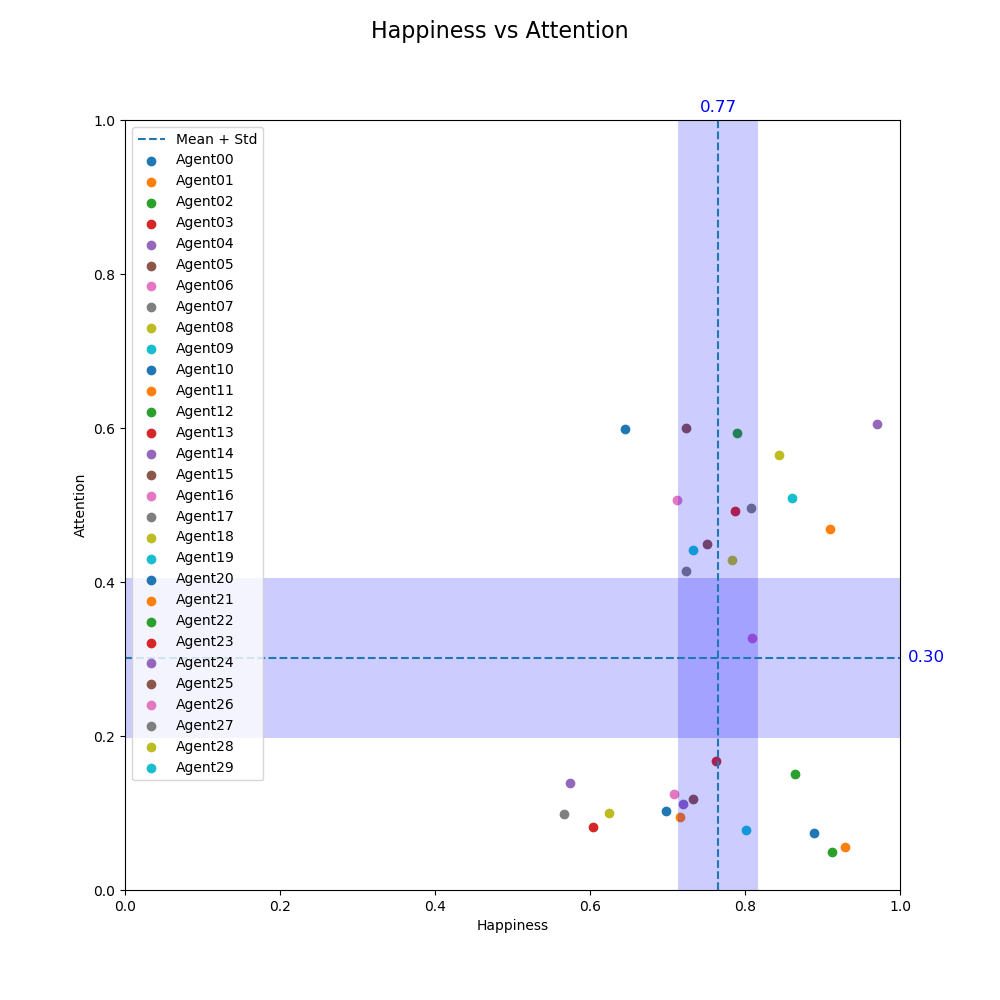
\includegraphics[width=500pt]{results/ADHD-VeryHigh/HA-Plot}
    \caption{HA Plot for first instance}
\end{figure}

\begin{figure}[H]
    \centering
    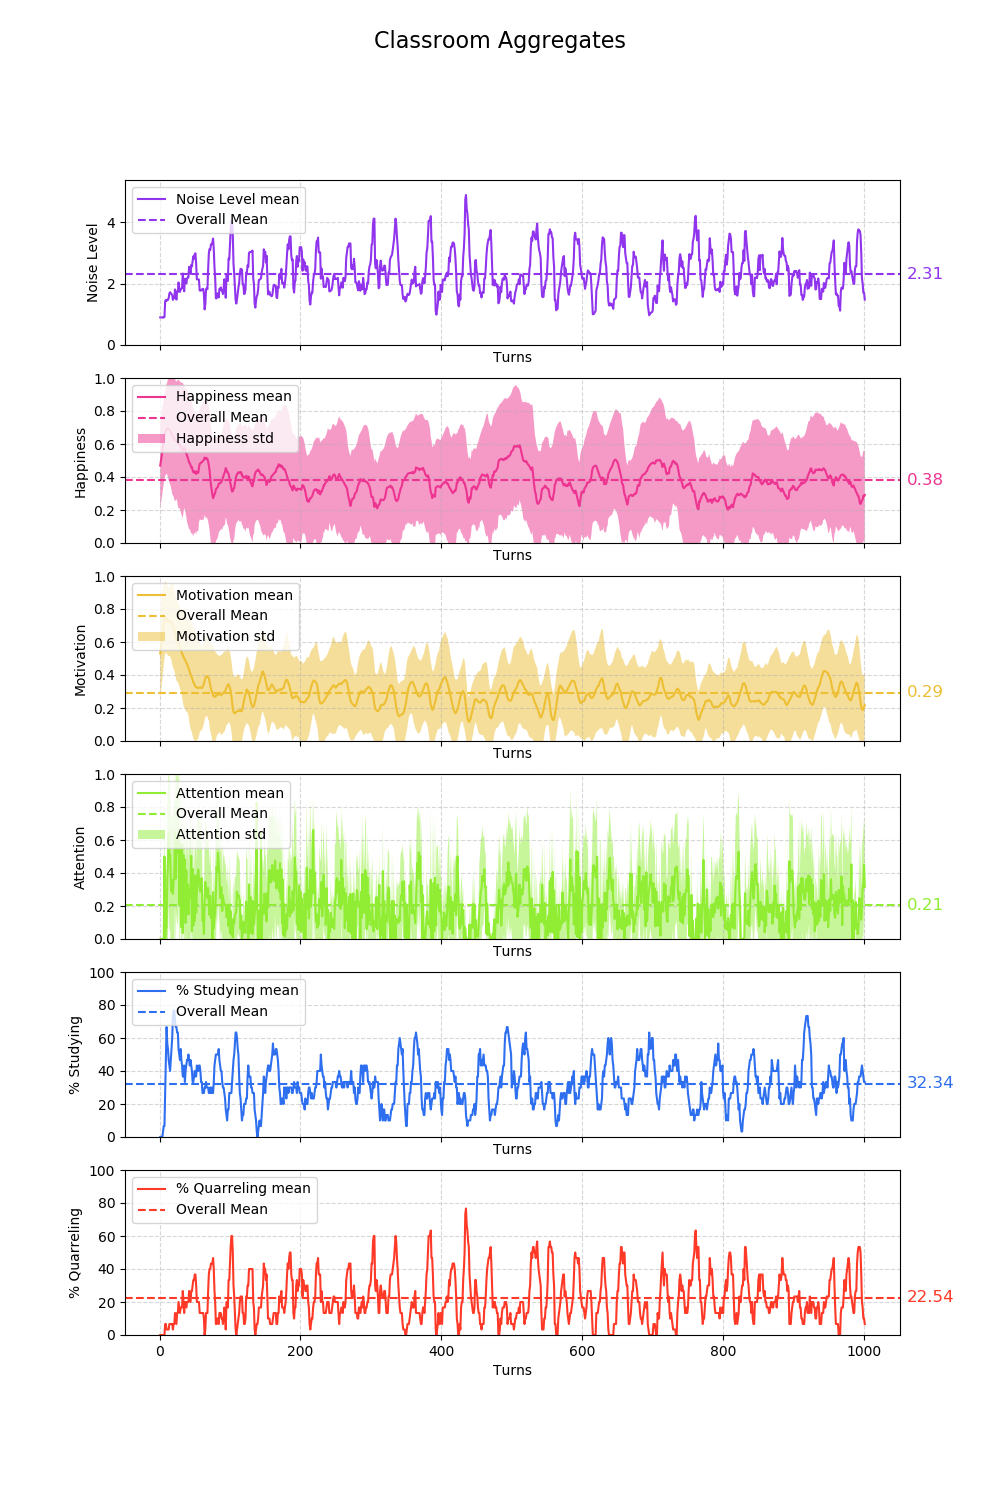
\includegraphics[width=400pt]{results/ADHD-VeryHigh/ClassroomAggregates}
    \caption{Classroom aggregates for first instance}
\end{figure}


%%%%%%%%%%%%%%%%%%%%%%%%%%%%%%%%%%%%%%%%%%%%%%%%%%%%%%%%%%%%%%%%%%%%%%%%%%%%%%%%
\subsection{ADHD-None}

\begin{figure}[H]
    \centering
    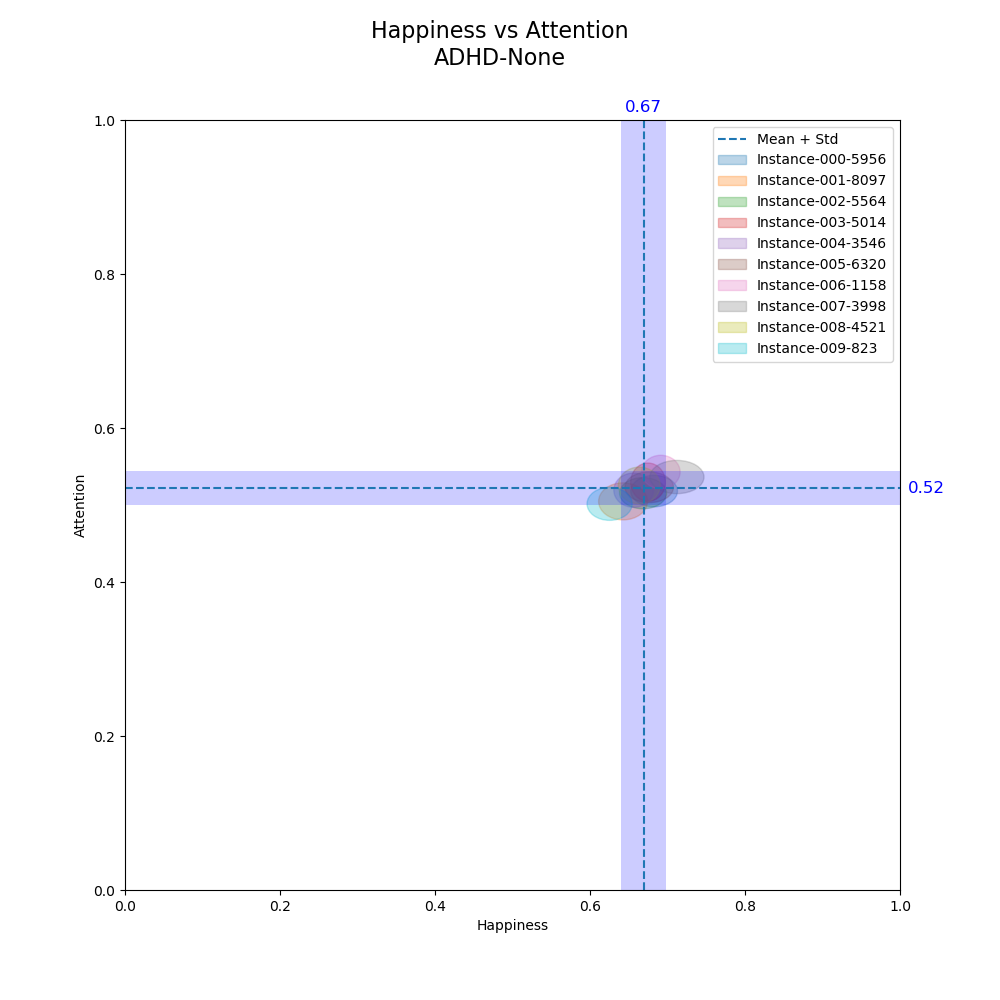
\includegraphics[width=500pt]{results/ADHD-None/Experiment_summary-AgentStd}
    \caption{HA Plot for complete experiment}
\end{figure}

\begin{figure}[H]
    \centering
    \includegraphics[width=500pt]{results/ADHD-None/HA-Plot}
    \caption{HA Plot for first instance}
\end{figure}

\begin{figure}[H]
    \centering
    \includegraphics[width=400pt]{results/ADHD-None/ClassroomAggregates}
    \caption{Classroom aggregates for first instance}
\end{figure}


%%%%%%%%%%%%%%%%%%%%%%%%%%%%%%%%%%%%%%%%%%%%%%%%%%%%%%%%%%%%%%%%%%%%%%%%%%%%%%%%
\subsection{ADHD-Medium-Ambitious}

\begin{figure}[H]
    \centering
    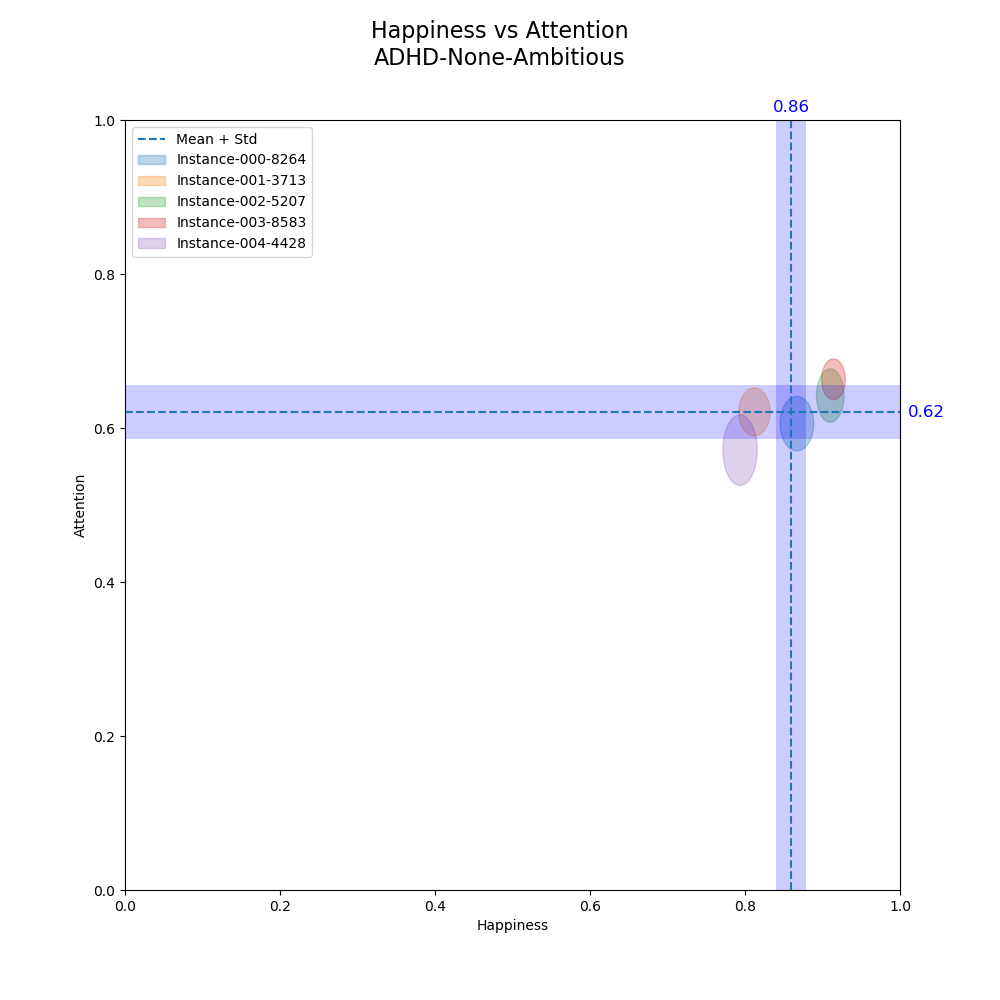
\includegraphics[width=500pt]{results/ADHD-Medium-Ambitious/Experiment_summary-AgentStd}
    \caption{HA Plot for complete experiment}
\end{figure}

\begin{figure}[H]
    \centering
    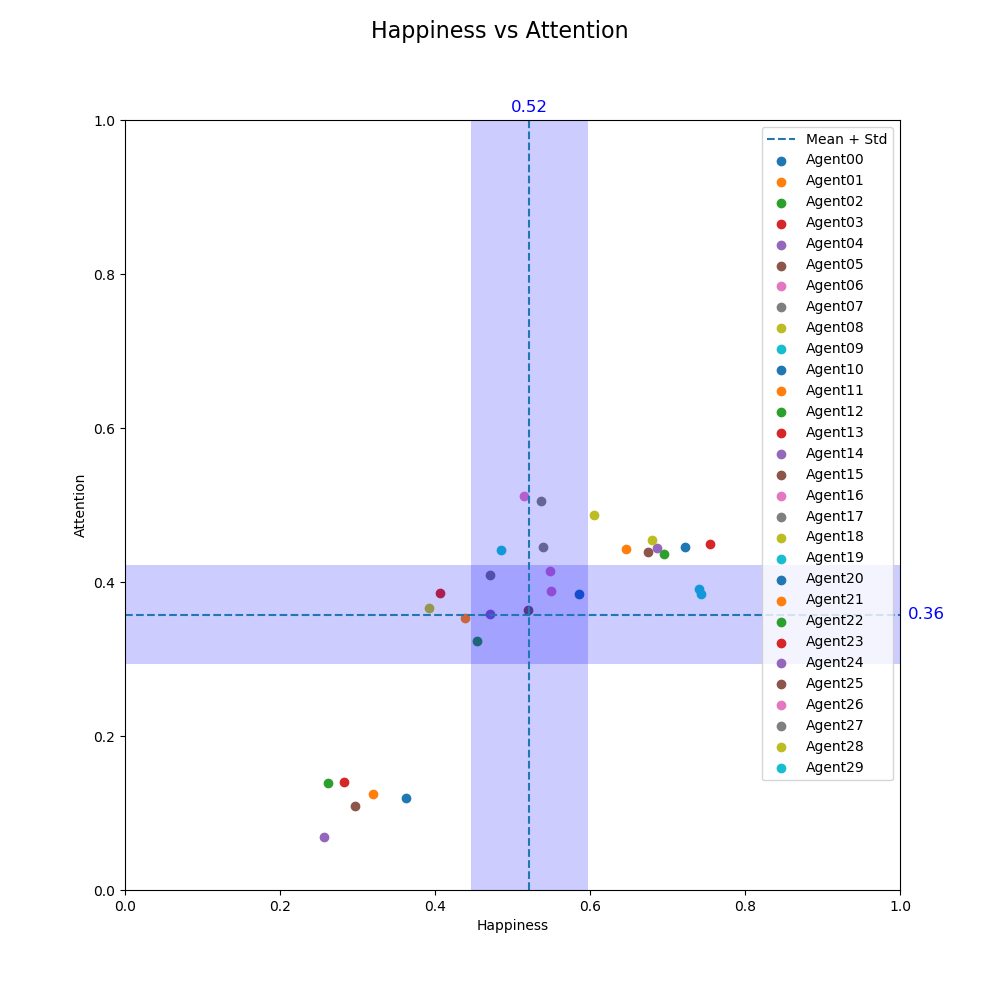
\includegraphics[width=500pt]{results/ADHD-Medium-Ambitious/HA-Plot}
    \caption{HA Plot for first instance}
\end{figure}

\begin{figure}[H]
    \centering
    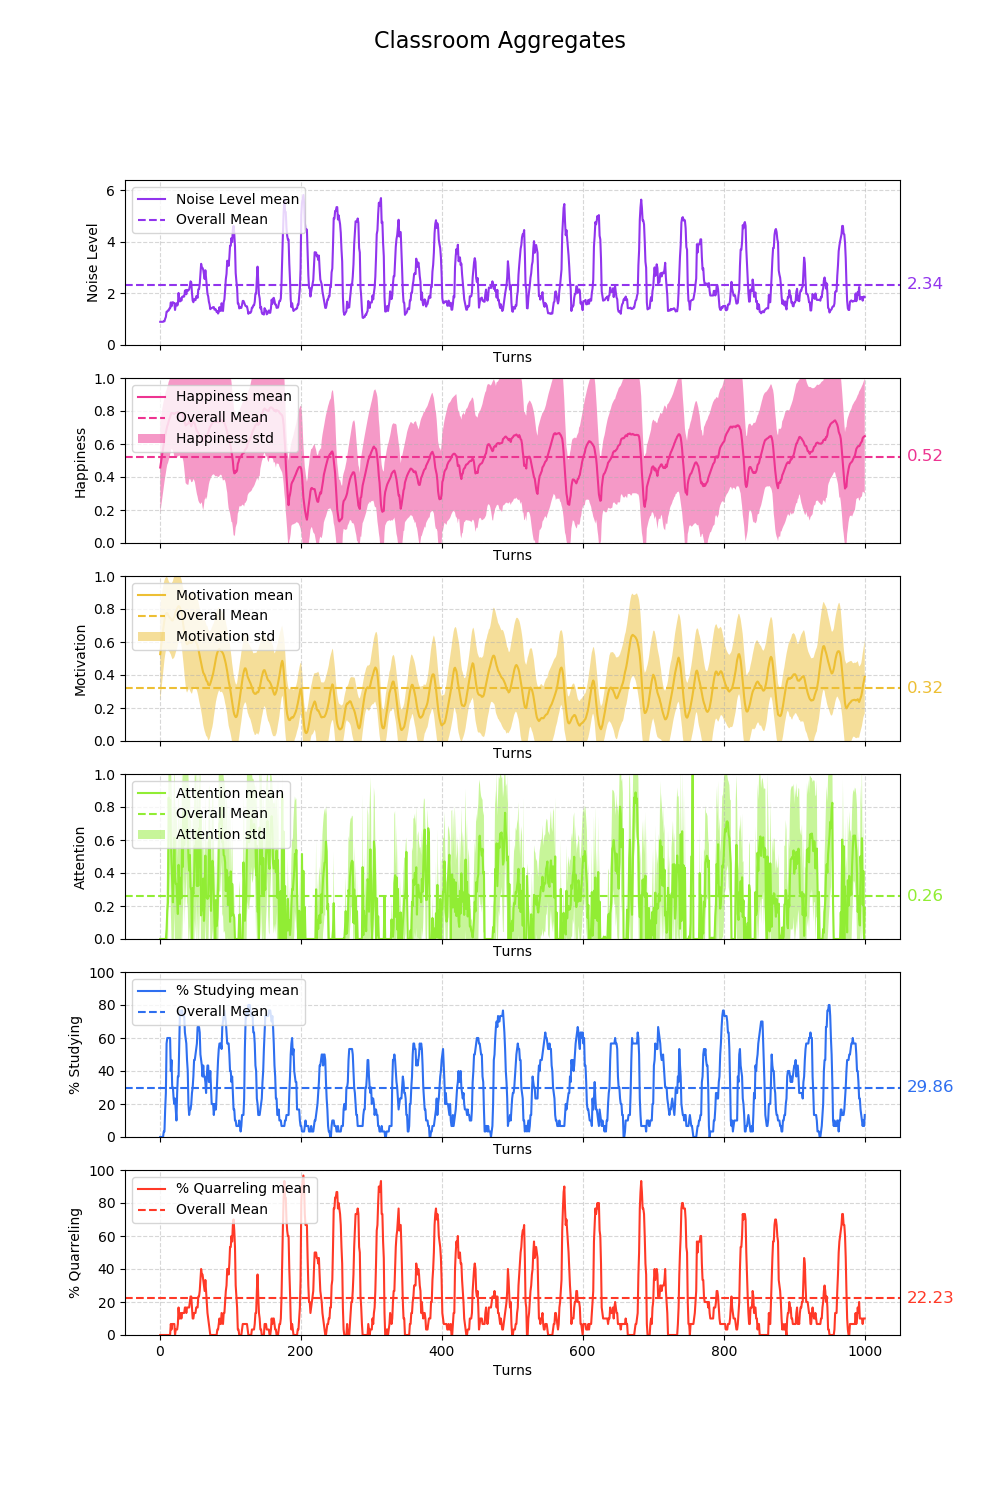
\includegraphics[width=400pt]{results/ADHD-Medium-Ambitious/ClassroomAggregates}
    \caption{Classroom aggregates for first instance}
\end{figure}

%%%%%%%%%%%%%%%%%%%%%%%%%%%%%%%%%%%%%%%%%%%%%%%%%%%%%%%%%%%%%%%%%%%%%%%%%%%%%%%%
\subsection{ADHD-None-Ambitious}

\begin{figure}[H]
    \centering
    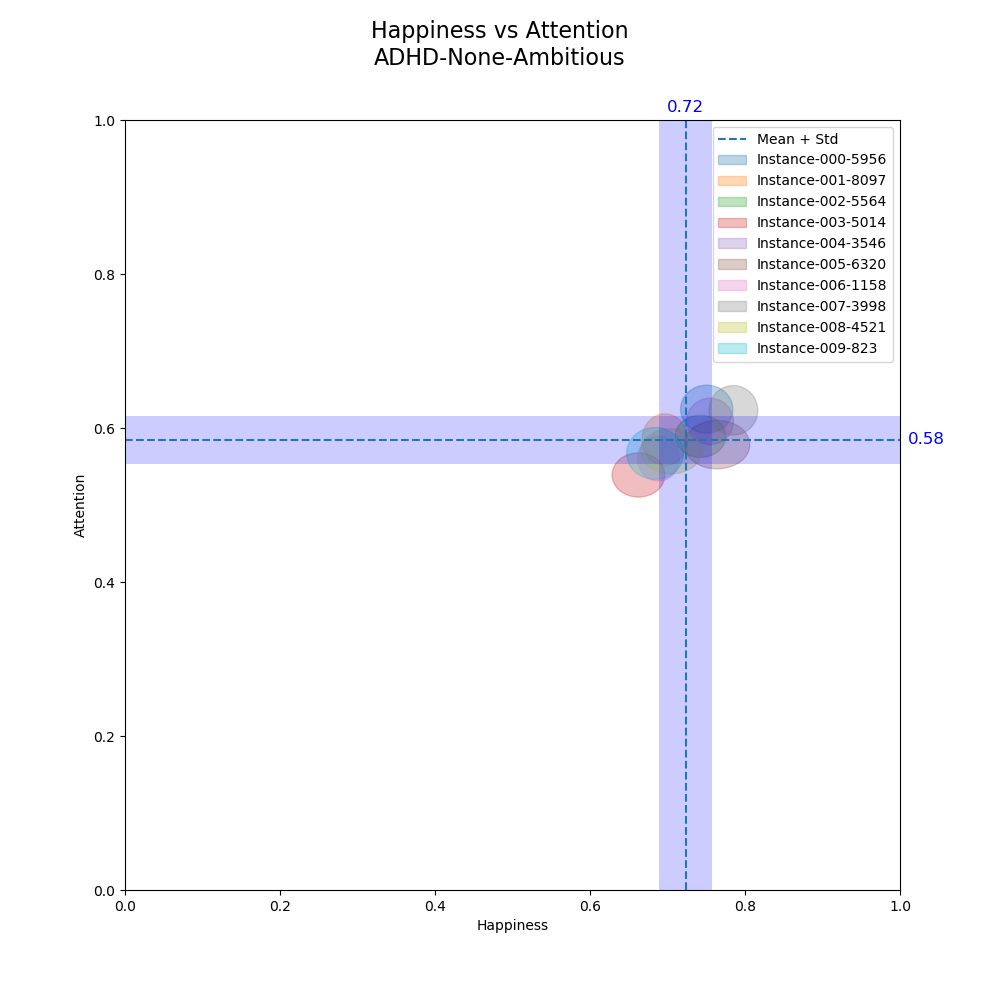
\includegraphics[width=500pt]{results/ADHD-None-Ambitious/Experiment_summary-AgentStd}
    \caption{HA Plot for complete experiment}
\end{figure}

\begin{figure}[H]
    \centering
    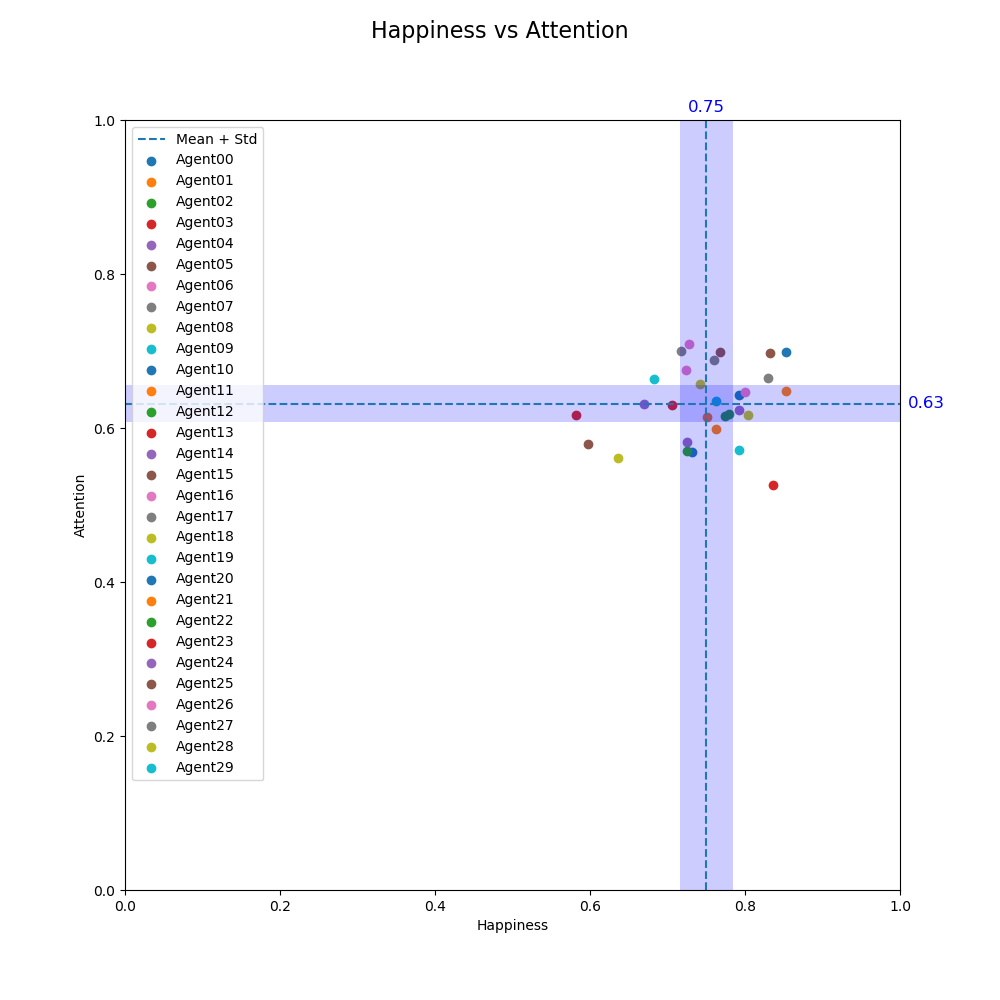
\includegraphics[width=500pt]{results/ADHD-None-Ambitious/HA-Plot}
    \caption{HA Plot for first instance}
\end{figure}

\begin{figure}[H]
    \centering
    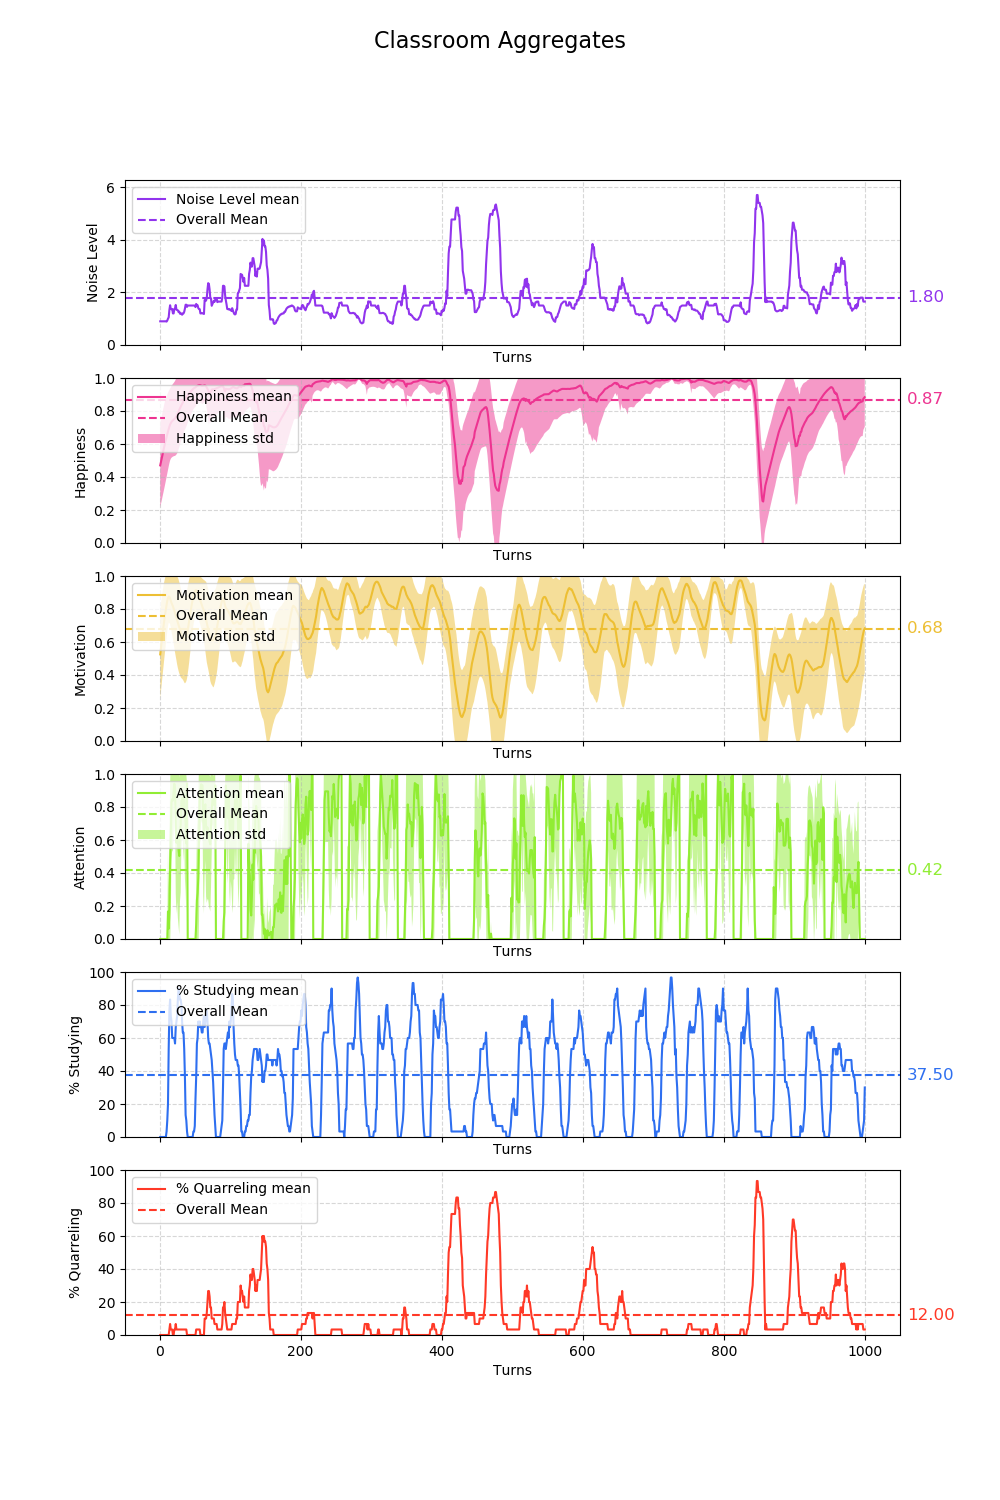
\includegraphics[width=400pt]{results/ADHD-None-Ambitious/ClassroomAggregates}
    \caption{Classroom aggregates for first instance}
\end{figure}

%%%%%%%%%%%%%%%%%%%%%%%%%%%%%%%%%%%%%%%%%%%%%%%%%%%%%%%%%%%%%%%%%%%%%%%%%%%%%%%%
\subsection{Random}

\begin{figure}[H]
    \centering
    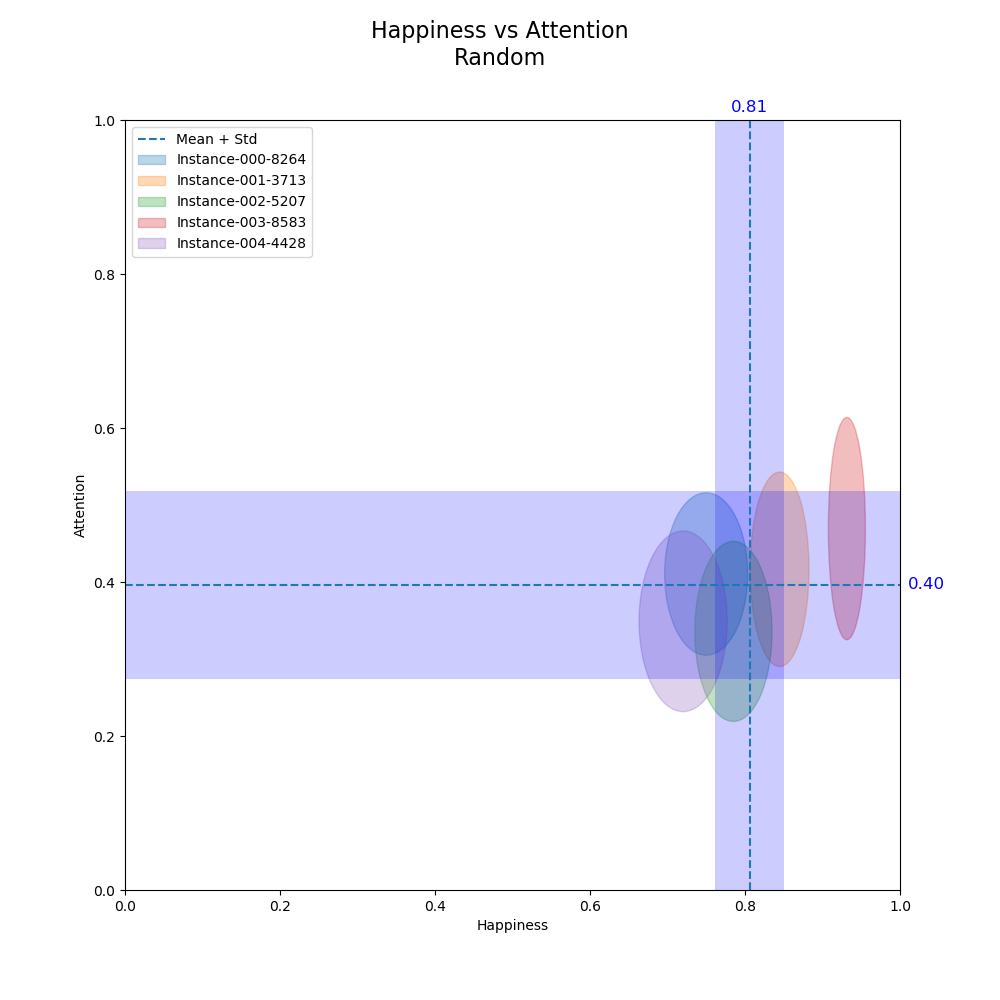
\includegraphics[width=500pt]{results/Random/Experiment_summary-AgentStd}
    \caption{HA Plot for complete experiment}
\end{figure}

\begin{figure}[H]
    \centering
    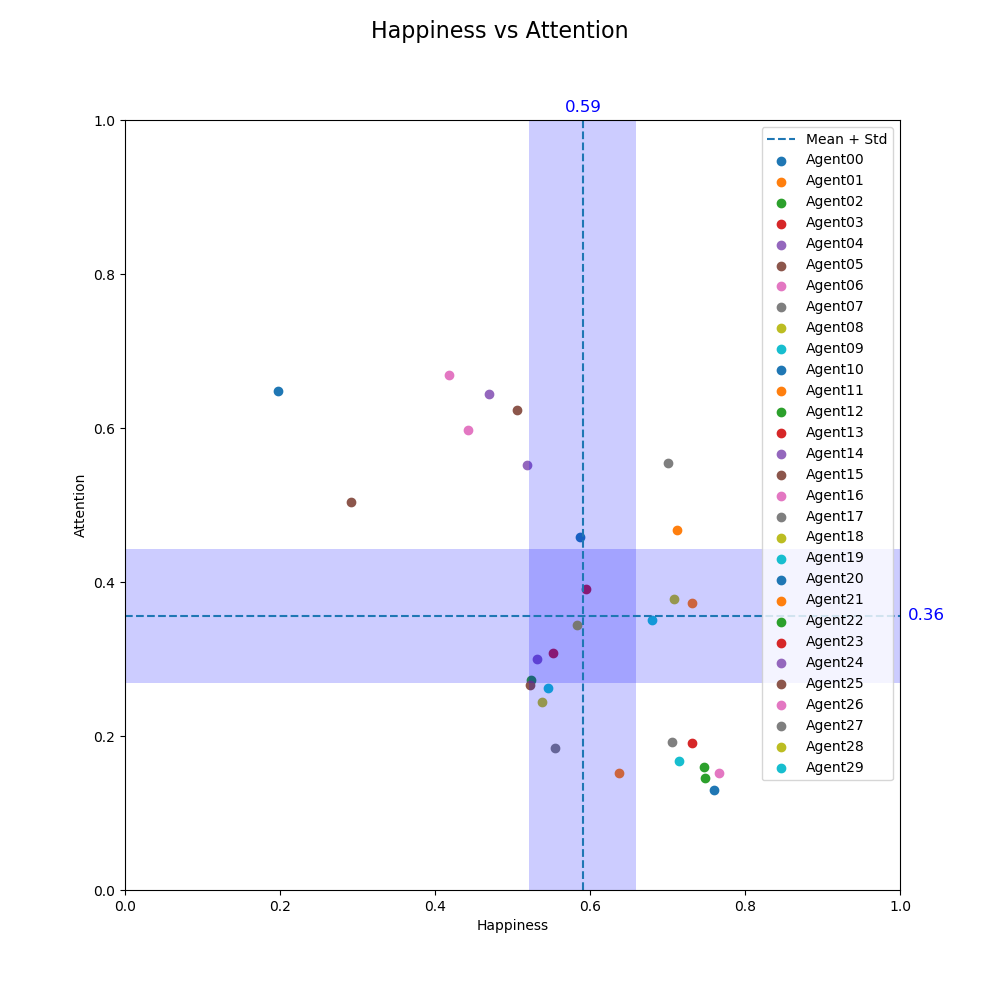
\includegraphics[width=500pt]{results/Random/HA-Plot}
    \caption{HA Plot for first instance}
\end{figure}

\begin{figure}[H]
    \centering
    \includegraphics[width=400pt]{results/ADHD-None/ClassroomAggregates}
    \caption{Classroom aggregates for first instance}
\end{figure}

[EOF]


\end{document}





















